%%%%%%%%%%%%%%%%%%%%%%%%%%%%%%%%%%%%%%%%%%%%%%%%%%%%%%%%%%%%%%%%%%%%%%%%%%%%%%%%
%% Plantilla de memoria en LaTeX para la ETSIT - Universidad Rey Juan Carlos
%%
%% Por Gregorio Robles <grex arroba gsyc.urjc.es>
%%     Grupo de Sistemas y Comunicaciones
%%     Escuela Técnica Superior de Ingenieros de Telecomunicación
%%     Universidad Rey Juan Carlos
%% (muchas ideas tomadas de Internet, colegas del GSyC, antiguos alumnos...
%%  etc. Muchas gracias a todos)
%%
%% La última versión de esta plantilla está siempre disponible en:
%%     https://github.com/gregoriorobles/plantilla-memoria
%%
%% Para obtener PDF, ejecuta en la shell:
%%   make
%% (las imágenes deben ir en PNG o JPG)

%%%%%%%%%%%%%%%%%%%%%%%%%%%%%%%%%%%%%%%%%%%%%%%%%%%%%%%%%%%%%%%%%%%%%%%%%%%%%%%%

\documentclass[a4paper, 12pt]{book}
%\usepackage[T1]{fontenc}

\usepackage[a4paper, left=2.5cm, right=2.5cm, top=3cm, bottom=3cm]{geometry}
\usepackage{times}
\usepackage[utf8]{inputenc}
\usepackage[spanish]{babel} % Comenta esta línea si tu memoria es en inglés
\usepackage{url}
%\usepackage[dvipdfm]{graphicx}
\usepackage{graphicx}
\usepackage{float}  %% H para posicionar figuras
\usepackage[nottoc, notlot, notlof, notindex]{tocbibind} %% Opciones de índice
\usepackage{latexsym}  %% Logo LaTeX
\usepackage{subfig}

\title{Memoria del Proyecto}
\author{David González Endrinal}

\renewcommand{\baselinestretch}{1.5}  %% Interlineado

\begin{document}

\renewcommand{\refname}{Bibliografía}  %% Renombrando
\renewcommand{\appendixname}{Apéndice}

%%%%%%%%%%%%%%%%%%%%%%%%%%%%%%%%%%%%%%%%%%%%%%%%%%%%%%%%%%%%%%%%%%%%%%%%%%%%%%%%
% PORTADA

\begin{titlepage}
\begin{center}
\includegraphics[scale=0.8]{img/URJ_logo_Color_POS.png}

\vspace{1.75cm}

\Large
GRADO EN INGENIERÍA EN TELEMÁTICA

\vspace{0.4cm}

\large
Curso Académico 2021/2022

\vspace{0.8cm}

Trabajo Fin de Grado

\vspace{2.5cm}

\LARGE
Aplicación de Web Progresiva (PWA) y optimización de la asistencia a seminarios de la URJC

\vspace{4cm}

\large
Autor : David González Endrinal \\
Tutor : Dr. Gregorio Robles Martínez
\end{center}
\end{titlepage}

\newpage
\mbox{}
\thispagestyle{empty} % para que no se numere esta pagina


%%%%%%%%%%%%%%%%%%%%%%%%%%%%%%%%%%%%%%%%%%%%%%%%%%%%%%%%%%%%%%%%%%%%%%%%%%%%%%%%
%%%% Para firmar
\clearpage
\pagenumbering{gobble}
\chapter*{}

\vspace{-4cm}
\begin{center}
\LARGE
\textbf{Trabajo Fin de Grado}

\vspace{1cm}
\large
Aplicación de Web Progresiva (PWA) y optimización de la asistencia a seminarios de la URJC

\vspace{1cm}
\large
\textbf{Autor :} David González Endrinal \\
\textbf{Tutor :} Dr. Gregorio Robles Martínez

\end{center}

\vspace{1cm}
La defensa del presente Trabajo Fin de Grado se realizó el día \qquad$\;\,$ de \qquad\qquad\qquad\qquad \newline de 2021, siendo calificada por el siguiente tribunal:


\vspace{0.5cm}
\textbf{Presidente:}

\vspace{1.2cm}
\textbf{Secretario:}

\vspace{1.2cm}
\textbf{Vocal:}


\vspace{1.2cm}
y habiendo obtenido la siguiente calificación:

\vspace{1cm}
\textbf{Calificación:}


\vspace{1cm}
\begin{flushright}
Fuenlabrada, a \qquad$\;\,$ de \qquad\qquad\qquad\qquad de 2021
\end{flushright}

%%%%%%%%%%%%%%%%%%%%%%%%%%%%%%%%%%%%%%%%%%%%%%%%%%%%%%%%%%%%%%%%%%%%%%%%%%%%%%%%
%%%% Dedicatoria

\chapter*{}
\pagenumbering{Roman} % para comenzar la numeracion de paginas en números romanos
\begin{flushright}
\textit{Dedicado a \\
mis padres, mis hermanas, mi abuelo y mis sobrinos}
\end{flushright}

%%%%%%%%%%%%%%%%%%%%%%%%%%%%%%%%%%%%%%%%%%%%%%%%%%%%%%%%%%%%%%%%%%%%%%%%%%%%%%%%
%%%% Agradecimientos

\chapter*{Agradecimientos}
%\addcontentsline{toc}{chapter}{Agradecimientos} % si queremos que aparezca en el índice
\markboth {AGRADECIMIENTOS}{AGRADECIMIENTOS}
En primer lugar quiero dar gracias a mi familia. En especial a mis padres quienes han estado conmigo desde el primer minuto, con un apoyo incondicional en todo momento, dándome ánimos en momentos en los que yo no los encontraba y los que me han dado la oportunidad de formarme durante toda mi vida. A mis hermanas, quienes se han alegrado tanto como yo en los momentos en los que aprobaba, mostraban ilusión por mis logros y las que me han aconsejado siempre buscando lo mejor para mí. A mi abuelo, que siempre ha tenido palabras de ánimo en todo momento que ha durado esta andadura universitaria.

	No hay palabras suficientes de agradecimiento por el apoyo que siempre he sentido y por demostrarme que podía con ello, este título es, en gran medida, gracias a vosotros.

	También quiero dar las gracias a mi tutor y profesor, Gregorio Robles, por darme la oportunidad de realizar este proyecto, de su ayuda y el interés mostrado durante la realización del mismo.
A todos los demás profesores que durante todos estos años han contribuido en mi formación.

	Por último, a todos los amigos que durante estos años universitarios han compartido conmigo sus dias, los buenos y los no tan buenos, con los que he podido forjar una gran amistad.

	\vspace{5mm} %5mm vertical space
	¡Gracias!


%%%%%%%%%%%%%%%%%%%%%%%%%%%%%%%%%%%%%%%%%%%%%%%%%%%%%%%%%%%%%%%%%%%%%%%%%%%%%%%%
%%%% Resumen

\chapter*{Resumen}
%\addcontentsline{toc}{chapter}{Resumen} % si queremos que aparezca en el índice
\markboth{RESUMEN}{RESUMEN} % encabezado

	Este proyecto consiste en la realización de una Aplicación de Web Progresiva (PWA en inglés, \emph{Progressive Web Applications}) que facilite los docentes el proceso de ofrecer a los alumnos los cursos/seminarios y jornadas tecnológicas que se imparten o tineen lugar en la Universidad durante el curso académico.
	
	Esta aplicación y todo su desarrollo se enmarca dentro del modelo cliente-servidor, donde por un lado tendremos por parte del cliente la PWA y por parte del servidor toda la administración y gestión de los contenidos que contendrá dicha aplicación.
	
	Para el desarrollo de la parte servidor se han utilizado diferentes entornos y lenguajes, destacando Python, Node y MongoDB para la gestión y almacenamiento en bases de datos.
	
	Con la creación de esta aplicación se intenta, por el lado docente, buscar una eficiencia a la hora de repartir y adjudicar las distintas aulas de las que se dispone para la realización de los distintos cursos y seminarios, por otro lado, por el lado de los alumnos, se busca tener un entorno de fácil manejo y simpleza a la hora de informarse, apuntarse y obtener los créditos correspondientes de dichos cursos y seminarios.

%%%%%%%%%%%%%%%%%%%%%%%%%%%%%%%%%%%%%%%%%%%%%%%%%%%%%%%%%%%%%%%%%%%%%%%%%%%%%%%%
%%%% Resumen en inglés

\chapter*{Summary}
%\addcontentsline{toc}{chapter}{Summary} % si queremos que aparezca en el índice
\markboth{SUMMARY}{SUMMARY} % encabezado

This project consists of the realization of a Progressive Web Application (PWA) that will help and facilitate the teachers the process of offering the students the courses / seminars and technological conferences that will be taught at the University during the course.
This application and all its development is framed within the client-server model, where, on the one hand, we will have the PWA on the part of the client and on the part of the server all the administration and management of the contents that said application will contain.
For the development of the server part, different environments and languages have been used, highlighting Python, Node and MongoDB for management and storage in databases.
With the creation of this application, an attempt is made, on the teaching side, to seek efficiency when distributing and allocating the different classrooms available to carry out the different courses and seminars, on the other hand, on the side of The students seek to have an environment that is easy to use and simple when it comes to obtaining information, signing up and obtaining the corresponding credits for said courses and seminars.


%%%%%%%%%%%%%%%%%%%%%%%%%%%%%%%%%%%%%%%%%%%%%%%%%%%%%%%%%%%%%%%%%%%%%%%%%%%%%%%%
%%%%%%%%%%%%%%%%%%%%%%%%%%%%%%%%%%%%%%%%%%%%%%%%%%%%%%%%%%%%%%%%%%%%%%%%%%%%%%%%
% ÍNDICES %
%%%%%%%%%%%%%%%%%%%%%%%%%%%%%%%%%%%%%%%%%%%%%%%%%%%%%%%%%%%%%%%%%%%%%%%%%%%%%%%%

% Las buenas noticias es que los índices se generan automáticamente.
% Lo único que tienes que hacer es elegir cuáles quieren que se generen,
% y comentar/descomentar esa instrucción de LaTeX.

%%%% Índice de contenidos
\tableofcontents 
%%%% Índice de figuras
\cleardoublepage
%\addcontentsline{toc}{chapter}{Lista de figuras} % para que aparezca en el indice de contenidos
\listoffigures % indice de figuras
%%%% Índice de tablas
%\cleardoublepage
%\addcontentsline{toc}{chapter}{Lista de tablas} % para que aparezca en el indice de contenidos
%\listoftables % indice de tablas


%%%%%%%%%%%%%%%%%%%%%%%%%%%%%%%%%%%%%%%%%%%%%%%%%%%%%%%%%%%%%%%%%%%%%%%%%%%%%%%%
%%%%%%%%%%%%%%%%%%%%%%%%%%%%%%%%%%%%%%%%%%%%%%%%%%%%%%%%%%%%%%%%%%%%%%%%%%%%%%%%
% INTRODUCCIÓN %
%%%%%%%%%%%%%%%%%%%%%%%%%%%%%%%%%%%%%%%%%%%%%%%%%%%%%%%%%%%%%%%%%%%%%%%%%%%%%%%%

\cleardoublepage
\chapter{Introducción}
\label{sec:intro} % etiqueta para poder referenciar luego en el texto con~\ref{sec:intro}
\pagenumbering{arabic} % para empezar la numeración de página con números

El siguiente trabajo consta de la realización de una aplicación web progresiva (PWA) que ayudará y facilitara a los docentes el proceso de ofrecer a los alumnos los cursos/seminarios y jornadas tecnológicas que se impartirán en la Universidad durante el curso.


\section{Contexto}
\label{sec:contexto}
La herramienta propuesta en este TFG nace de la necesidad por parte de la Universidad Rey Juan Carlos y más concretamente del administrador/profesor encargado de gestionar todo lo relaccionado con las charlas y seminarios que en ella se ofrecen.

Está principalmente orientada hacia los alumnos, que son en definitiva las personas que más uso harán de la misma, en cuanto a la parte web, supondrá una herramienta de fácil manejo donde ver estos horarios, apuntarse a ellos y obtener los créditos correspondientes por acudir a cada uno de ellos.

Por parte de la Universidad, y más concretamente del administrador o encargado de las charlas, agilizará y le quitará gran carga de trabajo, facilitando la gestión y adjudicación de los certificados que se entregarán a los usuarios finales de la misma.

La motivación para realizar este proyecto es para introducir, más si cabe, las nuevas tecnologías y la agilidad que éstas nos proporcionan dentro del entorno universitario, en su parte backend, destaca en la optimización de la gestión de las salas disponibles en la universidad en función de los alumnos apuntados a cada uno de estos seminarios.

Es un proyecto muy centrado en la automaticación de procesos, guardando la seguridad que se requiere en cuantos asuntos de gestión universitaria se refiere, facilitando y agilizando las gestiones tanto a alumnos como a la propia universidad.


%%%%%%%%%%%%%%%%%%%%%%%%%%%%%%%%%%%%%%%%%%%%%%%%%%%%%%%%%%%%%%%%%%%%%%%%%%%%%%%%
%%%%%%%%%%%%%%%%%%%%%%%%%%%%%%%%%%%%%%%%%%%%%%%%%%%%%%%%%%%%%%%%%%%%%%%%%%%%%%%%
% OBJETIVOS %
%%%%%%%%%%%%%%%%%%%%%%%%%%%%%%%%%%%%%%%%%%%%%%%%%%%%%%%%%%%%%%%%%%%%%%%%%%%%%%%%

\cleardoublepage % empezamos en página impar
\chapter{Objetivos} % título del capítulo (se muestra)
\label{chap:objetivos} % identificador del capítulo (no se muestra, es para poder referenciarlo)

\section{Objetivo general} % título de sección (se muestra)
\label{sec:objetivo-general} % identificador de sección (no se muestra, es para poder referenciarla)

La realización de este trabajo de fin de grado consiste en crear una Aplicación Web Progresiva o PWA que proporcionara a alumnos y a docentes una herramienta de fácil manejo con la que estar informado y gestionar los distintos cursos/seminarios y jornadas tecnológicas que se impartirán en la Universidad durante el curso.


\section{Objetivos específicos}
\label{sec:objetivos-especificos}

\begin{itemize}
  \item Automatizar el reparto de las aulas durante los días y las horas disponibles
  \item Informar al docente o administrador de la aplicación del número de alumnos apuntados a los distintos cursos/seminarios y jornadas
  \item Informar a los alumnos del horario de los distintos cursos/seminarios y jornadas tecnológicas
  \item Gestionar (apuntado y borrando) a los alumnos interesados en los seminarios disponibles
\end{itemize}


\section{Planificación temporal}
\label{sec:planificacion-temporal}

\begin{figure}
  \centering
  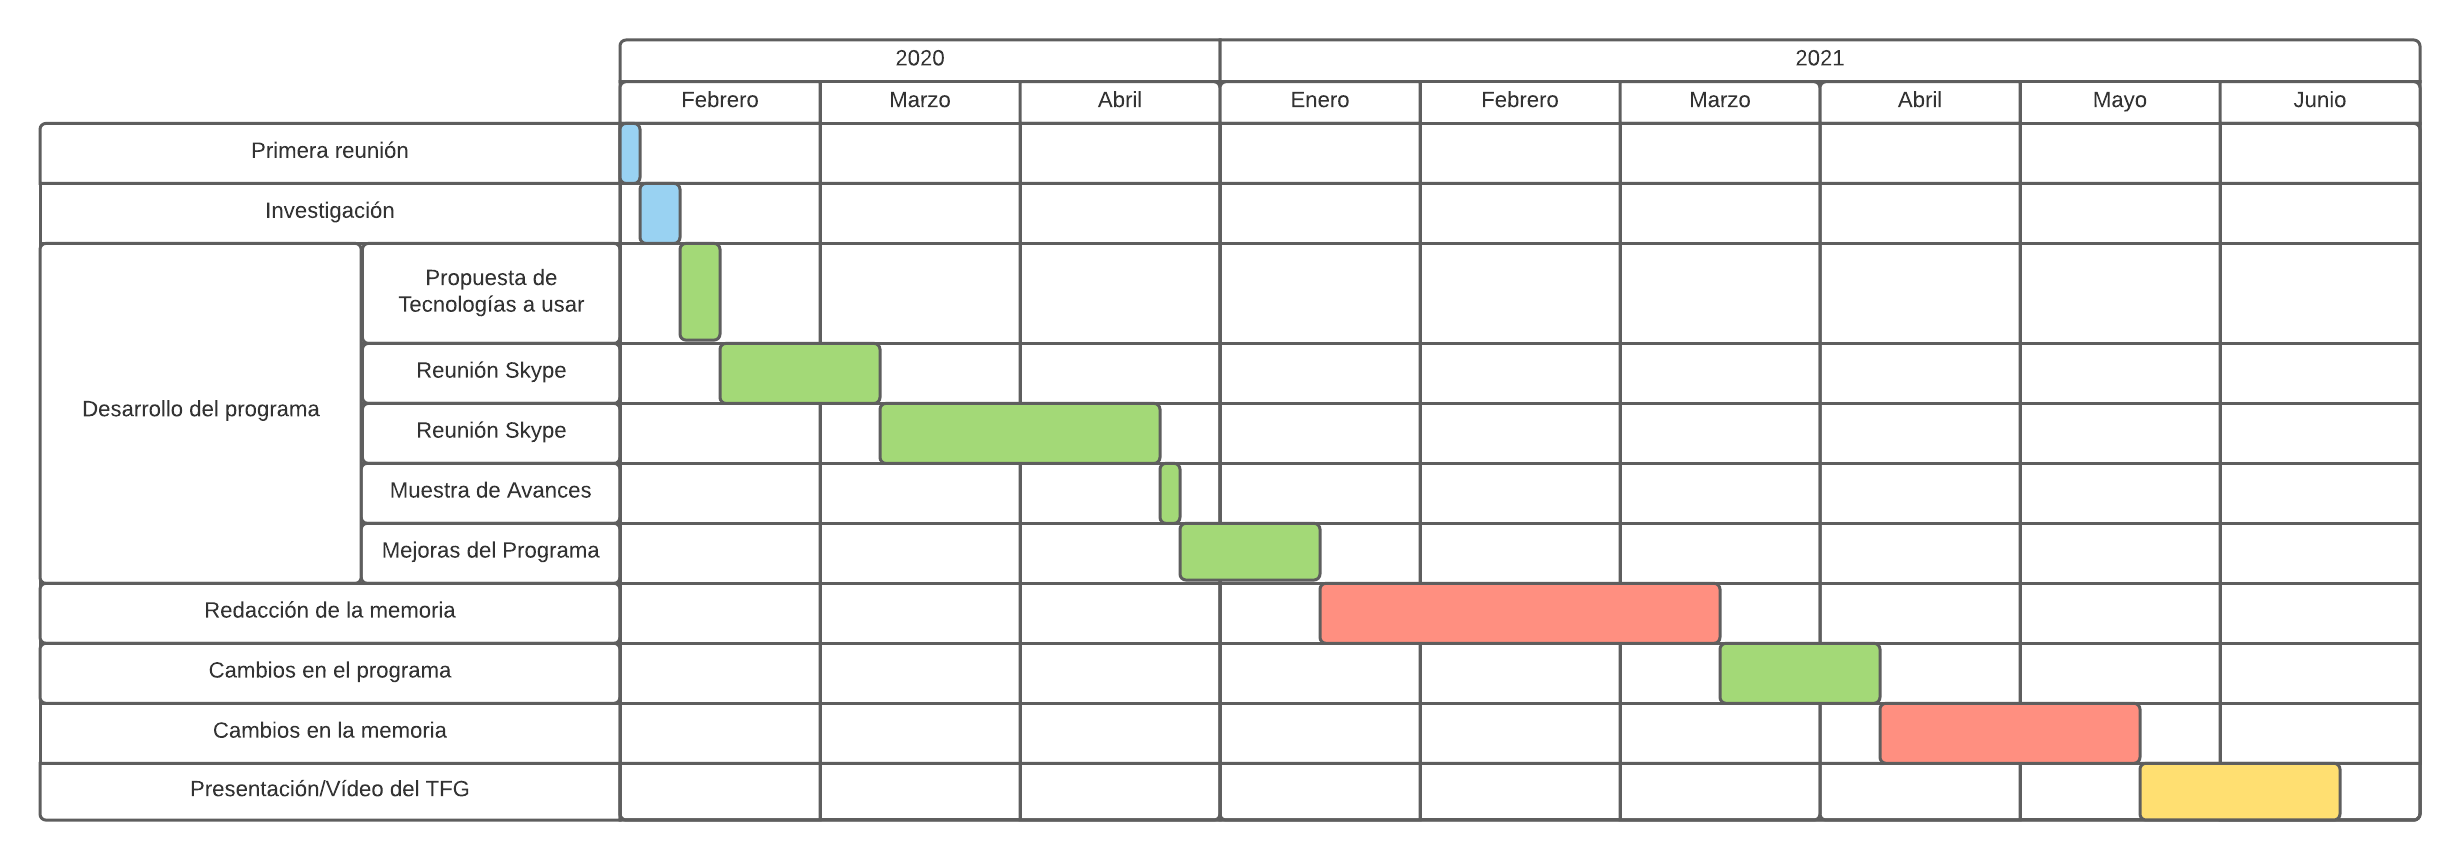
\includegraphics[width=16cm, keepaspectratio]{img/diagrama.png}
  \caption{Diagrama de Gantt del desarrollo del TFG.}\label{fig:diagrama}
\end{figure}

Antes incluso de saber la temática del TFG o sobre que iba a tratar, tenía claro las tecnologías que quería usar. En esos momentos estaba adentrándome en el mundo front con Angular y el desarrollo de aplicaciones Web.

La primera toma de contacto con Gregorio fué a traves del correo de la URJC, en el que por medio del mismo comenté mi preferencia a hacer el TFG con él, allá por febrero del 2020. En la primera reunión Gregorio me propuso varios temas sobre los que podía enfocar mi TFG, todos sobre desarrollo Web pero con un requisito claro, debería funcionar y estar optimizados para utilizarlos en dispositivos móviles.

Después de esa reunión pase los siguientes dias investigando sobre que tipo de aplicacón debería tratar, y fué ahi cuando decidí hacer una aplicación de web progresiva (PWA), habría leído sobre ellas, las conocía un poco y vi que era una gran oportunidad de aprender y desarrollar algo nuevo para mí. En la siguiente reunion del mismo mes de febrero presenté esta tecnología a Gregorio y fue cuando empezó el desarrollo de la misma.

Entre todo el 2020 y alternando con mi trabajo a jornada completa fuí desarrollando el proyecto, teniendo durante este tiempo 3 reuniones via Skype con Gregorio para mostrar los avances de la aplicación, preguntar algunas dudas y recibir consejos de por donde podría enforcar el desarrollo.

En Enero de 2021 tuve la ultima reunión para hablar del desarrollo de la aplicación, ya estaba terminada con la integración de algunos puntos y funciones que me pedía Gregorio y fué en ese momento cuando recibí la validación por su parte y pasé a redactar la memoria.

Durante la redaccion de esta memoria seguí teniendo un contacto muy directo con mi tutor, subia borradores de la memoria a un repositorio y él se encargaba de leerlo, darme consejos y modificarlo si así lo veía oportuno.

Por último con la  memoría terminada, retoque un poco el código a petición de Gregorio como ha ido haciendo a lo largo de este TFG mostrando una participación en el muy activa y siempre estando dispuesto a colaborar.

Ya estaban terminadas las dos partes principales de este TFG, la aplicacion propiamente programada y la presente memoria, fue aquí cuando decidir hacer una presentación de este TFG de cara a la defensa del mismo.


%%%%%%%%%%%%%%%%%%%%%%%%%%%%%%%%%%%%%%%%%%%%%%%%%%%%%%%%%%%%%%%%%%%%%%%%%%%%%%%%
%%%%%%%%%%%%%%%%%%%%%%%%%%%%%%%%%%%%%%%%%%%%%%%%%%%%%%%%%%%%%%%%%%%%%%%%%%%%%%%%
% ESTADO DEL ARTE %
%%%%%%%%%%%%%%%%%%%%%%%%%%%%%%%%%%%%%%%%%%%%%%%%%%%%%%%%%%%%%%%%%%%%%%%%%%%%%%%%

\cleardoublepage
\chapter{Estado del arte}
\label{chap:estado}

A continuación se detallan las tecnologías utilizadas en el desarrollo del proyecto.



\section{Angular} 
\label{sec:Angular}
Angular es un framework para aplicaciones web desarrollado en TypeScript (lenguaje del que hablaremos más adelante), de código abierto, mantenido por Google, que se utiliza para crear y mantener aplicaciones web de una sola página. Su objetivo es aumentar las aplicaciones basadas en navegador con capacidad de Modelo Vista Controlador (MVC), en un esfuerzo para hacer que el desarrollo y las pruebas sean más fáciles.

Entre sus virtudes se destacan:
\begin{itemize}
\item La posibilidad de utilizar templates declarativos, aplicar inyecciones de dependencias y crear componentes reutilizables.

\item Es modular, por lo cual se basa en un core y en módulos que permiten acceder a más características cuando es necesario. Permite crear componentes, razón por la cual se destaca en la reutilización de los elementos.


\item Ejecuta la primera vista de tu aplicación en node.js, .NET, PHP, y otros servidores para renderizado de forma casi instantánea obteniendo solo HTML y CSS. También abre posibilidades para la optimización del SEO (Search Engine Optimization) del sitio, incluyendo configuración.

\item Son aplicaciones que cargan rápidamente gracias al nuevo enrutador de componentes. Este ofrece una división automática de códigos para que los usuarios solo carguen el código necesario para procesar la vista que solicitan.

\item Por último, dentro de las cosas que debemos tener en cuenta de Angular, es que nuestros proyectos deben ser compilados para traducirlos en una aplicación Web que podamos publicar. Este compilador ha sido mejorado a partir de Angular 5, permitiendo ahora compilación incremental y logrando como resultado que los re-build sean más rápidos.
\end{itemize}

A continuación destacamos dos paquetes npm que son importantes y sobre los que gira gran parte de este proyecto de fin de grado:

\subsection{@zxing/ngx-scanner v.3.0.0}
\label{subsec:@zxing/ngx-scanner}
Paquete con el que por medio de una simple linea de código permite a nuestra aplicación angular (PWA) activar la cámara de nuestro dispositivo y pudiendo leer códigos QR o Códigos de barras simples obteniendo información de los mismos. 
	En este proyecto daremos uso a este paquete a la hora de validar nuestra presencia en cualquiera de las charlas o seminarios en los que estemos inscritos y así poder certificar que hemos asistido a ellos para más tarde poder pedir el certificado con los créditos correspondientes.

\subsection{@angular/pwa v.0.1101.1}
\label{subsec:@angular/pwa}
Es el paquete principal que usaremos para convertir nuestra aplicación Angular en una Aplicación de Web Progresiva (PWA), mediante el comando \textit{ng add @angular/pwa} se añadirán una serie de archivos y se modificarán otros existentes para poder realizar este cambio, dichas modificaciones son:

\begin{enumerate}
\item Se agregará el paquete \textit{@angular/service-workerpaquete} al proyecto

\item Habilita la compatibilidad con la compilación del trabajador de servicios en la CLI.

\item Importa y registra al trabajador del servicio en el módulo de la aplicación.

\item Actualiza el archivo \textit{index.html} incluyendo un enlace para agregar el archivo \textit{manifest.webmanifest}.

\item Instala archivos de iconos para admitir la aplicación web progresiva (PWA) instalada.

\item Crea el archivo de configuración del service worker \textit{llamado ngsw-config.json}, que especifica los comportamientos de almacenamiento en caché y otras configuraciones.
\end{enumerate}


\section{Typescript}
\label{sec:Typescript}
Typescript es un superset de JavaScript, decimos que una tecnología es un superset de un lenguaje de programación, cuando puede ejecutar programas de la tecnología, Typescript en este caso, y del lenguaje del que es el superset, JavaScript en este mismo ejemplo.

	Esto permite que se pueda integrar Typescript en proyectos existentes de JavaScript sin tener que reimplementar todo el código del proyecto en Typescript, de hecho, es común que existan proyectos que introduzcan tanto Typescript como JavaScript.
	
	La principal característica de Typescript es el tipado estático, decimos que un lenguaje es de tipado estático cuando no es necesario definir las variables antes de su uso. Esto implica que la tipificación estática tiene que ver con la declaración explícita (o inicialización) de las variables antes de que se empleen.


\section{HTML}
\label{sec:HTML}
HTML son las siglas de HyperText Markup Language, se trata del lenguaje estándar utilizado para la creación de páginas web. Fue creado por Tim Berners-Lee en los años ochenta. Es un lenguaje de marcas, esto quiere decir que para indicar la estructura del documento se utilizan etiquetas. Al ser un estándar, todos los navegadores leen e interpretan el lenguaje HTML y lo presentan de un modo similar.

\section{CSS}
\label{sec:CSS}
CSS son las siglas de Cascading Style Sheets, es un lenguaje que permite establecer la apariencia de un documento escrito mediante un lenguaje de marcas. CSS permite asociar reglas a los elementos que aparecen en una página web, las reglas indican como debe representarse el contenido de esos elementos.

\section{Bootstrap}
\label{sec:Bootstrap}
Bootstrap es un framework front-end que permite la construcción de páginas web adaptativas. Se trata de un software de código abierto creado en el año 2011 por Mark Otto y Jacob Thornton, empleados de Twitter.

	Bootstrap ha evolucionado desde ser un proyecto enteramente basado en CSS hasta incluir múltiples plugins JavaScript e iconos junto con formularios y botones. Presenta una cuadrícula de doce columnas y 940px de ancho.

	La creación de páginas web mediante Bootstrap se simplifica al disponer de elementos pre-definidos fácilmente incluibles en cualquier página web, tales como menús desplegables, botones, iconos, ventanas emergentes, etc.

\section{Node} 
\label{sec:Node}
	Node.js es un entorno JavaScript que nos permite ejecutar en el servidor, de manera asíncrona, con una arquitectura orientada a eventos y basado en el motor V8 de Google.
	
	El motor V8 de Google compila Javascript en código máquina nativo en vez de interpretarlo en el navegador, consiguiendo así una velocidad mucho más alta, además de la alta velocidad de ejecución, Node.js dispone del Bucle de Eventos (Event Loop), que permitirá gestionar enormes cantidades de clientes de forma asíncrona. Tradicionalmente para trabajar de forma asíncrona las aplicaciones se valían de la programación basada en hilos (programming threaded applications), pero esto supone la utilización (normalmente ineficaz) de un espacio de memoria que va escalando a medida que la cantidad de clientes conectados a nuestra aplicación aumenta.
	
	Node.js resuelve este problema cambiando la manera de realizar las conexiones con el servidor. En vez de generar un nuevo hilo E/S para cada cliente, cada conexión dispara la ejecución de un evento dentro del proceso del motor de Node. De este modo, Node permite que un solo servidor que lo ejecute pueda soportar decenas de miles de conexiones. Por lo tanto, si necesitamos gestionar grandes cantidades de conexiones no tendremos que ampliar el número de servidores.

	En conclusión, es una plataforma que agiliza y facilita las conexiones cliente servidor por lo que es una tecnología que avanza muy rápidamente y cada vez está más presente en el mercado.

\section{MongoDB} 
\label{sec:MongoDB}

Es una de las bases de datos noSQL y orientada a documentos que existen, esto quiere decir que en lugar de guardar los datos en registros, guarda los datos en documentos. Estos documentos son almacenados en BSON, que es una representación binaria de JSON. Una de las diferencias más importantes con respecto a las bases de datos relacionales, es que no es necesario seguir un esquema. Los documentos de una misma colección - concepto similar a una tabla de una base de datos relacional -, pueden tener esquemas diferentes.

	Aunque se suele decir que las bases de datos NoSQL tienen un ámbito de aplicación reducido, MongoDB se puede utilizar en muchos de los proyectos que desarrollamos en la actualidad, dos puntos a tener en cuenta sobre esta base de datos son:
	
	No existen las transacciones: Aunque nuestra aplicación puede utilizar alguna técnica para simular las transacciones, MongoDB no tiene esta capacidad. Solo garantiza operaciones atómicas a nivel de documento.

	No existen los JOINS: MongoDB esta destinado a proyectos en los que los datos no tengan que  ser estructurados en tablas y que tampoco tengamos que hacer relaciones entre ellas.


\section{Python} 
\label{sec:Python}
Python es un lenguaje de scripting desarrollado a principios de los noventa por Guido van Rossum, independiente de plataforma y orientado a objetos, preparado para realizar cualquier tipo de programa, desde aplicaciones Windows a servidores de red o incluso, páginas web. Entre sus muchas características destacamos:

\begin{itemize}
\item Multiplataforma: Hay versiones disponibles de Python en muchos sistemas informáticos distintos. Originalmente se desarrolló para Unix, aunque cualquier sistema es compatible con el lenguaje siempre y cuando exista un intérprete programado para él.

\item Interpretado: Quiere decir que no se debe compilar el código antes de su ejecución. En ciertos casos, cuando se ejecuta por primera vez un código, se producen unos bytecodes que se guardan en el sistema y que sirven para acelerar la compilación implícita que realiza el intérprete cada vez que se ejecuta el mismo código.

\item Interactivo: Python dispone de un intérprete por línea de comandos en el que se pueden introducir sentencias. Cada sentencia se ejecuta y produce un resultado visible, que puede ayudarnos a entender mejor el lenguaje y probar los resultados de la ejecución de porciones de código rápidamente.

\item Orientado a Objetos: La programación orientada a objetos está soportada en Python y ofrece en muchos casos una manera sencilla de crear programas con componentes reutilizables.

\item Gran cantidad de funciones y librerías: Dispone de muchas funciones incorporadas en el propio lenguaje, para el tratamiento de strings, números, archivos, etc. Además, existen muchas librerías que podemos importar en los programas para tratar temas específicos como la programación de ventanas o sistemas en red o cosas tan interesantes como crear archivos comprimidos en .zip.

\item Sintaxis clara: Por último, destacar que Python tiene una sintaxis muy visual, gracias a una notación identada (con márgenes) de obligado cumplimiento. Para separar las porciones de código en Python se debe tabular hacia dentro, colocando un margen al código que iría dentro de una función o un bucle. Esto ayuda a que todos los programadores adopten unas mismas notaciones y que los programas de cualquier persona tengan un aspecto muy similar.
\end{itemize}




%%%%%%%%%%%%%%%%%%%%%%%%%%%%%%%%%%%%%%%%%%%%%%%%%%%%%%%%%%%%%%%%%%%%%%%%%%%%%%%%
%%%%%%%%%%%%%%%%%%%%%%%%%%%%%%%%%%%%%%%%%%%%%%%%%%%%%%%%%%%%%%%%%%%%%%%%%%%%%%%%
% DISEÑO E IMPLEMENTACIÓN %
%%%%%%%%%%%%%%%%%%%%%%%%%%%%%%%%%%%%%%%%%%%%%%%%%%%%%%%%%%%%%%%%%%%%%%%%%%%%%%%%

\cleardoublepage
\chapter{Diseño e implementación}

A continuación se detalla el proyecto de Aplicación de Web Progresiva (PWA) del que trata este trabajo de fin de grado

\section{Arquitectura general} 
\label{sec:arquitectura}

Este proyecto gira en torno a la arquitectura software del modelo cliente-servidor, como se detalla en la figura~\ref{fig:arquitectura}. Destacamos la parte del cliente principalmente manejada por Angular y más concretamente la PWA y por otro lado, la parte del servidor controlada en su punto central por NodeJs, con una base de datos MongoDB y un par de programas desarrollados en python que ayudarán a la automatización, optimización y organización de las salas.
\begin{figure}
  \centering
  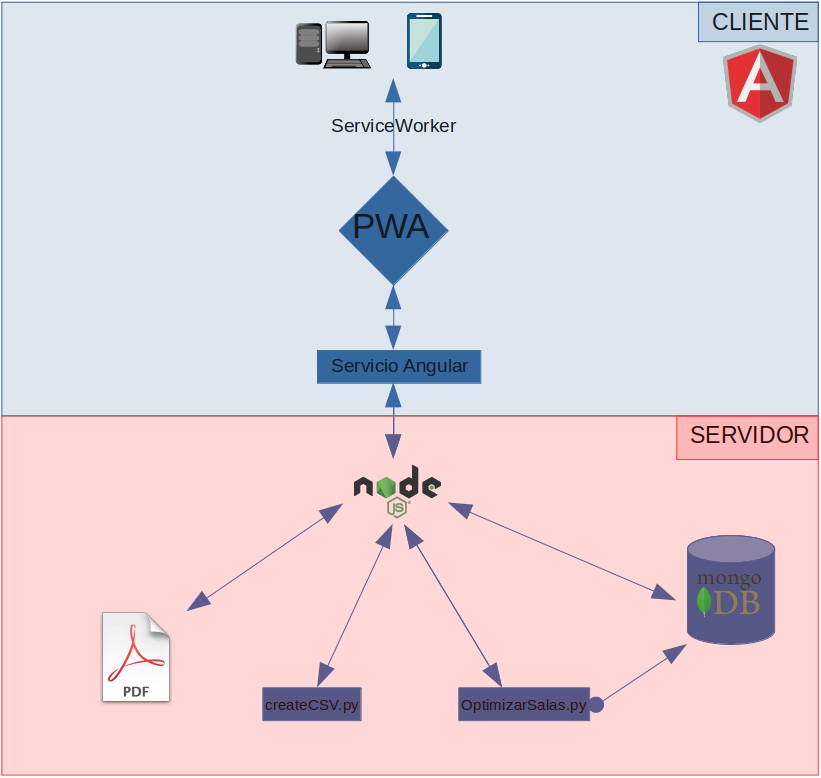
\includegraphics[width=10cm, keepaspectratio]{img/arquitectura.png}
  \caption{Arquitectura general.}\label{fig:arquitectura}
\end{figure}

 
\subsection{Cliente}
	En el lado del cliente tenemos toda la parte desarrollada con Angular, mas concretamente con el paquete \textit{@angular/pwa v.0.1101.1} al tratarse de una PWA y tratar con el framework Bootstrap permite que todas las pantallas de la aplicación sean \textit{responsive}, lo que quiere decir que estas pantallas se ajustarán automáticamente a la resolución del dispositivo en el que se muestran, centrado principalmente en dispositivos móviles llegándose a asemejar a una app nativa.
	
	Debido al uso de la cámara del dispositivo, los server workers proporcionados por el paquete \textit{@angular/pwa v.0.1101.1} y un login inicial de usuario (usuario y claves) es de obligado cumplimiento que la página se muestre con el protocolo seguro de transferencia de hipertexto (en inglés, Hypertext Transfer Protocol Secure o HTTPS)  para garantizar que la transferencia de datos no se vera comprometida en ningún momento y será seguro, esto se consigue con un certificado de clave pública para el servidor web.
	
	En las vistas del cliente diferenciamos dos variantes principales una vez que se hace login, para los usuarios que serán generalmente alumnos y para el administrador de la aplicación, este último tendrá unas vistas propias y unos privilegios por parte del servidor que no tendrá ningún otro usuario. Estos privilegios le permitirá modificar elementos de la base de datos, obtener información de todas las charlas, seminarios y de los alumnos apuntados a cada una de ellas.

	
\subsection{Servidor}
	En el lado del servidor se realiza el desarrollo back-end al completo, desde la recepción de peticiones HTTPS hasta el acceso a datos o la descarga de ellos en formato CSV o PDF.
	La parte central de este servidor gira en torno a NodeJs y mas concretamente en su framework Express que nos proporciona los mecanismos para poder manejar las peticiones HTTPS (get, post, put y delete) de los distintos usuarios. Una vez recibida una de estas peticiones, por medio del manejador proporcionado por express realizaremos una u otra acción, entre las principales de login, registro, getEvento entre otros, destacaremos dos:
	
\begin{itemize}
	\item \textbf{/getCreditoEventos}: Esta petición en concreto se encarga de recibir como parámetros strings el nombre, apellidos y el DNI del usuario, que por medio de la pestaña de \textit{certificado} y más concretamente apretando el botón \textit{``Recibir Créditos''} rellena una plantilla PDF suministrada por la URJC donde se adjudican al alumno los créditos correspondientes por asistir a una de estas charlas o seminarios que previamente se apuntó
	

	\item \textbf{/zip}: Esta petición solo es posible recibirla cuando es el administrador el que la requiere, se recibe como parámetros dos elementos, el primero el identificador del evento dentro de la base de datos y el nombre del evento. Esta petición lanzará un python llamado createCSV.py que se encarga de crear el CSV con los datos obtenidos de la base de datos y dejarlo en una ruta específica dentro del servidor, donde más tarde se recogerá y se mandara vía HTTPS al usuario administrador.

Esta petición en concreto tiene dos caminos:
\begin{itemize}
	\item  Si el administrador quiere un evento en concreto, el id del evento corresponderá a su identificador dentro de la base de datos devolverá un CSV que rellenará con los datos obtenidos de la base de datos en función de ese identificador recibido. 
	\item Si el administrador quiere obtener todos los eventos, el id del evento será 0, cuando obtenemos este identificador el servidor creara un .zip que contendrá varios CSV con los eventos en los que haya más de un alumno inscrito. Estos CSV tendrán el mismo formato y la misma información que el CSV devuelto en el caso anterior.
\end{itemize}
\end{itemize}


\section{Modelo de datos} 
\label{sec:modelo de datos}

\subsection{MongoDB}
	Para el almacenamiento de las distintas aulas disponibles, los alumnos inscritos y los horarios de las distintas charlas y seminarios tenemos los siguientes modelos de datos almacenados en la base da datos de MongoDB:
	
\begin{itemize}
	\item Eventos: En este Modelo de datos tendríamos almacenados JSON del con el formato que se puede apreciar en la figura~\ref{fig:mongoDBEventos}:
	\begin{figure}
  	\centering
  	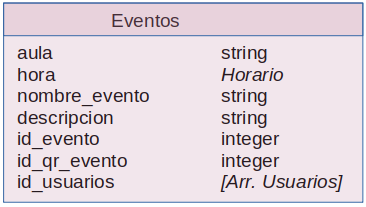
\includegraphics[width=10cm, keepaspectratio]{img/mongoDBEventos.png}
  	\caption{Modelo Eventos.}\label{fig:mongoDBEventos}
	\end{figure}
		\begin{itemize}
		\item Aula: Nombre correspondiente al aula donde se impartirá la charla o seminario almacenada en el Modelos de datos de \textit{Salas}
		\item Hora: Hora correspondiente a la que se impartirá la charla o seminario, corresponderá a una hora almacenada en el Modelo de datos de \textit{Horario}
		\item Nombre\_evento: Nombre correspondiente al Evento que se expondrá a la hora y en el aula especificado en los dos puntos anteriores
		\item Descripción: Descripción el evento presentado
		\item Id\_Evento: Identificador interno del evento presentado
		\item Id\_qr\_evento: Identificador del QR correspondiente al evento presentado
		\item Id\_usuarios: Array del mode de datos de \textit{Usuarios} donde se especifica los usuarios apuntados al evento presentado
		\end{itemize}
		
	\item Usuarios: En este Modelo de datos tendríamos almacenados JSON del con el formato que se aprecia en la figura~\ref{fig:mongoDBUsuarios}:
	\begin{figure}
  	\centering
  	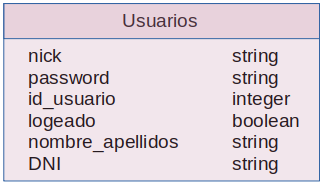
\includegraphics[width=10cm, keepaspectratio]{img/mongoDBUsuarios.png}
  	\caption{Modelo Usuarios.}\label{fig:mongoDBUsuarios}
	\end{figure}
		\begin{itemize}
		\item Nick: Nombre correspondiente al alumno reconocido internamente en la URJC
		\item Password: Contraseña encriptada en AES192
		\item Id\_usuario: Identificador interno del usuario
		\item Logueado: Indicador true (conectado) o false(desconectado) del usuario
		\item Nombre\_apellidos: Nombre y apellidos del Usuario
		\item DNI: DNI del Usuario
		\end{itemize}
	
	\item Salas En este Modelo de datos tendríamos almacenados JSON del con el formato que se puede apreciar en la figura~\ref{fig:mongoDBSalas}:
	\begin{figure}
  	\centering
  	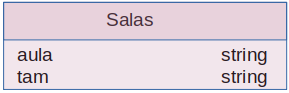
\includegraphics[width=10cm, keepaspectratio]{img/mongoDBSalas.png}
  	\caption{Modelo Salas.}\label{fig:mongoDBSalas}
	\end{figure}
	
	\begin{itemize}
		\item Aula: Nombre correspondiente al aula y como se la reconoce internamente en la URJC.
		\item Tam: Tamaño máximo de la sala.
	\end{itemize}
	
	\item Horario: En este Modelo de datos tendríamos almacenados JSON del con el formato de la siguiente figura~\ref{fig:mongoDBHorario}:
	\begin{figure}
  	\centering
  	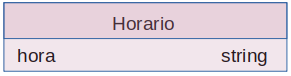
\includegraphics[width=10cm, keepaspectratio]{img/mongoDBHorario.png}
  	\caption{Modelo Salas.}\label{fig:mongoDBHorario}
	\end{figure}
	\begin{itemize}
		\item Hora: Horas disponibles para todas la aulas en los días especificados.
	\end{itemize}
\end{itemize}

\subsection{Registros de Alumnos y Eventos}
	Este apartado solo será visible por parte el administrador de la aplicación o del docente encargado en gestionar la semana cultural donde se impartan estas charlas y seminarios. Como vimos anteriormente, el administrador tiene la posibilidad de descargarse un archivo en formato CSV (comma-separated values, del inglés valores separados por comas) con toda la información de un Evento o de todos ellos, obteniendo un listado de los alumnos que se han apuntado a un determinado evento y que han validado su asistencia por medio de nuestra aplicación.
	El formato que tienen estos CSV corresponden a la figura~\ref{fig:CSVAlumnos}:
	\begin{figure}
  	\centering
  	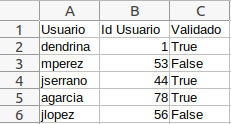
\includegraphics[width=10cm, keepaspectratio]{img/CSVAlumnos.png}
  	\caption{Modelo del archivo CSV.}\label{fig:CSVAlumnos}
	\end{figure}
	\begin{itemize}
		\item Usuario: Corresponde a un string almacenado en la base de datos de MongoDB con el formato de modelo de datos de \textit{Usuarios}
		\item Id\_usuario: String correspondiente campo id\_usuario del modelo de datos de \textit{Usuarios}
		\item True o False en el campo ``validado'' hace referencia a si el alumno ha asistido al evento y ha escaneado el código QR disponible al finalizar el mismo dando constancia así que asistió a él, campo a True, o por el contrario está apuntado pero no asistió a él siendo en este caso False el valor de este campo.
	\end{itemize}
	

\subsection{Plantilla documento de obtención créditos}
	El pdf que obtiene el alumno es un documento oficial de la Universidad Rey Juan Carlos en el que se le otorga un determinado número de créditos (fijados por el responsable de los seminarios o charlas) por acudir a las los seminarios o charlas que previamente se apuntó mediante la aplicación de la que estamos tratando en este TFG. La obtención de este certificado se hará de forma automática una vez que el alumno haya acudido a un número mínimo de seminarios fijados por el responsable de las mismas. 
	El formato que tendra el documento para la obteción de los créditos será el indicado en la siguiente figura~\ref{fig:pdfcreditos}:
	
\begin{figure}
  \centering
  
\includegraphics[width=10cm, keepaspectratio]{img/certificadoCreditos.png}
  \caption{Plantilla PDF créditos.}\label{fig:pdfcreditos}
\end{figure}

\begin{itemize}
		\item 1: Nombre del profesor encargado de los seminarios y charlas
		\item 2: Nombre del alumno al que se le otorgarán los créditos.
		\item 3: DNI del alumno
		\item 4: Fechas correspondientes a los días en los que tendrán lugar las charlas o seminarios
		\item 5: Número de créditos que obtendrá el alumno por asistir a los seminarios
		\item 6: Firma del profesor o responsable encargado de otorgar los créditos al alumno.
		\end{itemize}


\section{Diseño e implementación por funcionalidad } 

\subsection{Cliente}

\subsubsection{Login}
	La aplicación se integraŕa dentro de las aplicaciones de la Universidad Rey Juan Carlos para el uso tanto de profesores como de alumnos, es por ello por que guarda una estética distintiva de la universidad, con el uso de sus logos y colores, como podemos apreciar en la figura~\ref{fig:principalHome}:
	\begin{figure}
  	\centering
  	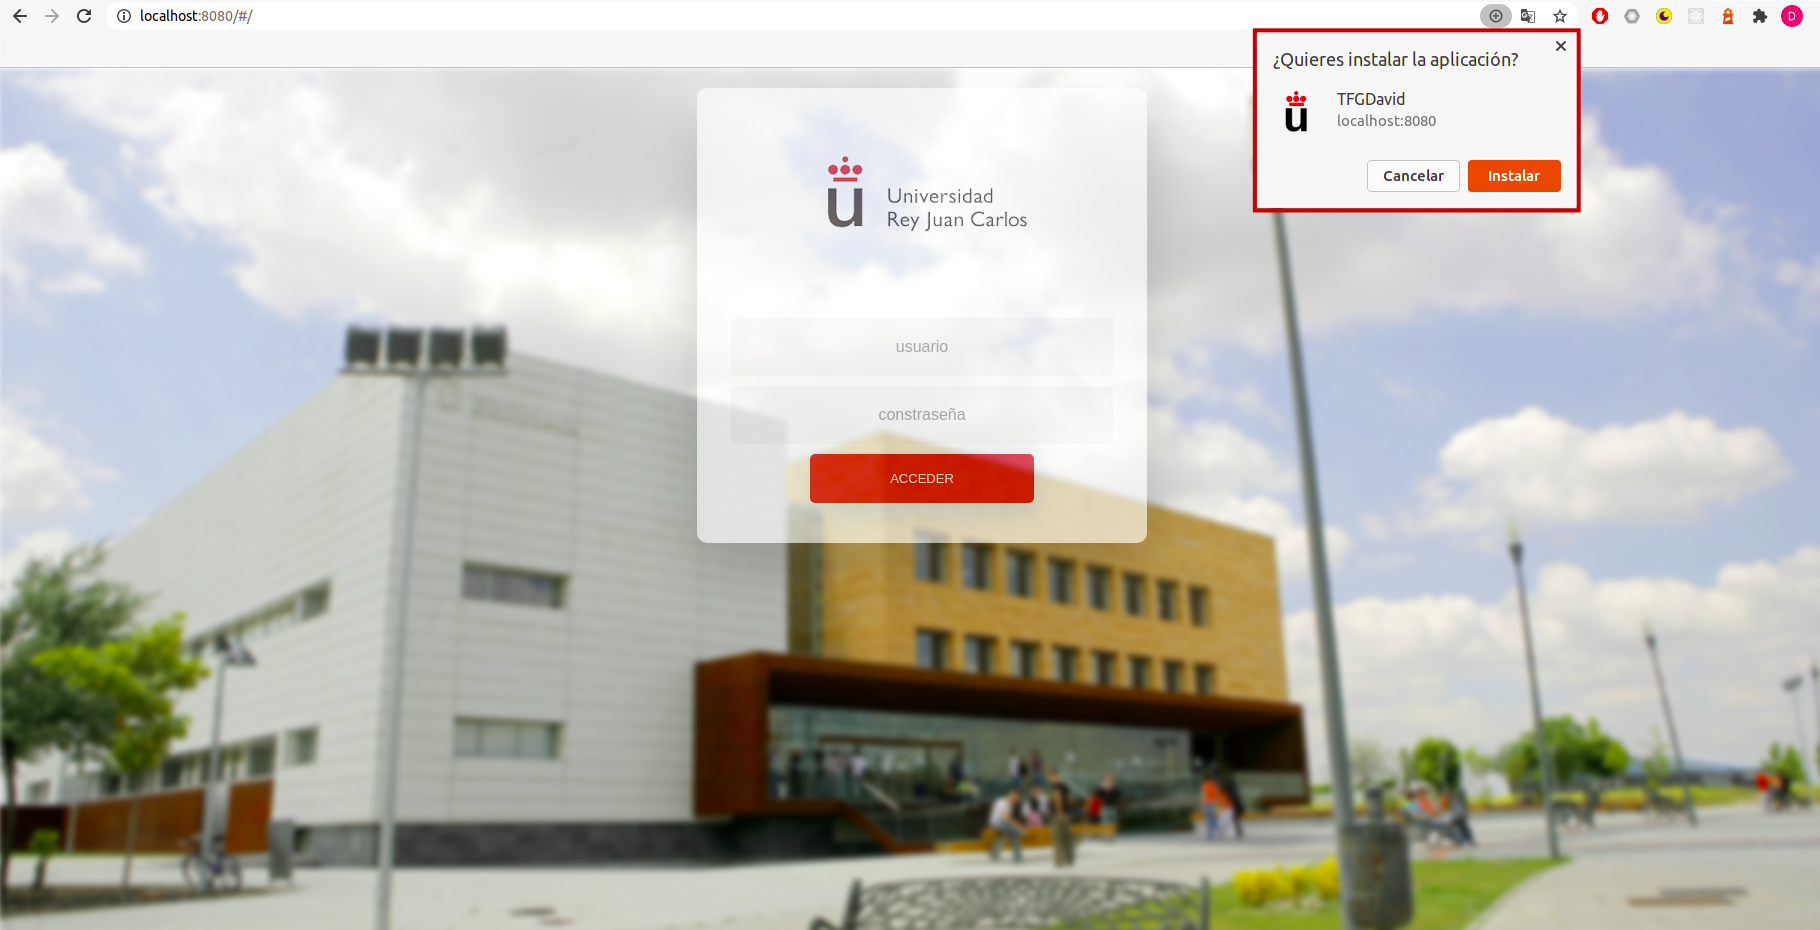
\includegraphics[width=16cm, keepaspectratio]{img/principalHome.png}
  	\caption{Página Login}\label{fig:principalHome}
	\end{figure}
La página de \textit{login} consta de un menú de login donde el usuario ingresará sus credenciales propias de la Universidad Rey Juan Carlos. En esta página destacamos dos puntos claves de por qué esta aplicación es una PWA.
	En primer lugar, tal y como se observa en la figura~\ref{fig:principalHome} el navegador tanto en ordenador como en dispositivos móviles nos da la opción de instalar la aplicación en nuestro dispositivo, creando un acceso directo a ella como si de una aplicación nativa android (en el caso móvil) o como una extensión chrome (en el caso de utilizar un navegador chrome en el ordenador) se tratase.
	En segundo lugar, como observamos en la figura~\ref{fig:principalWorker} la aplicación dispone también de un \textit{service worker}.
	
	\begin{figure}
  	\centering
  	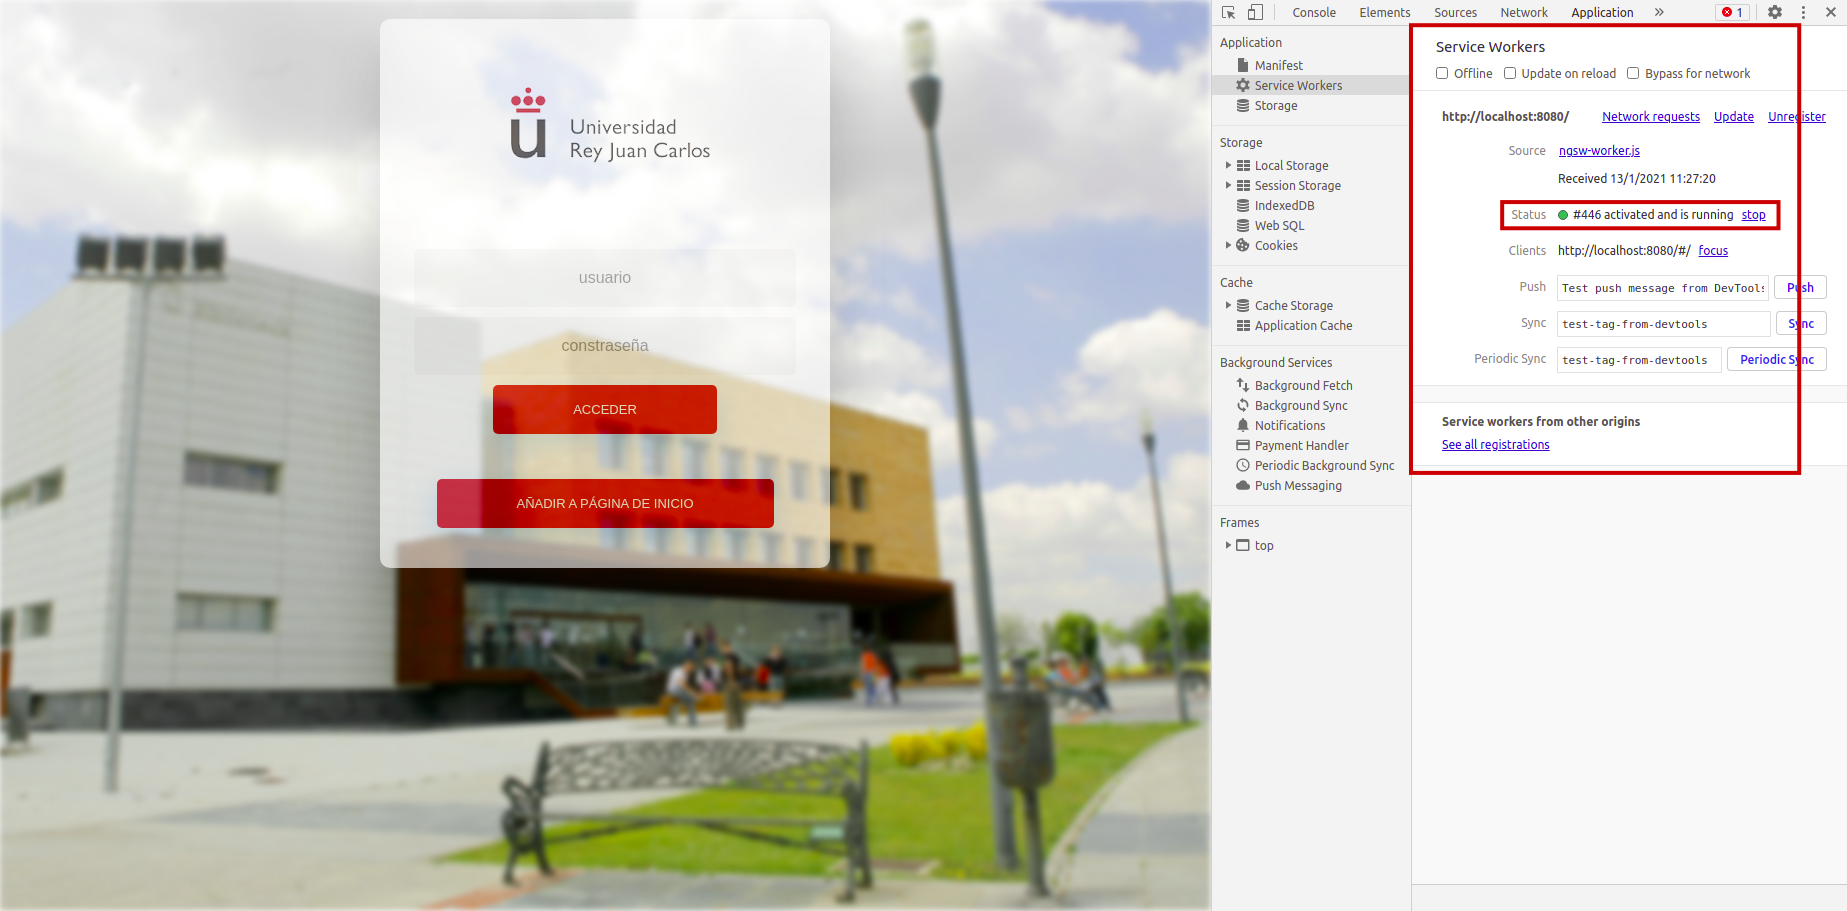
\includegraphics[width=16cm, keepaspectratio]{img/principalWorker.png}
  	\caption{Página Login}\label{fig:principalWorker}
	\end{figure}

	Un \emph{service worker} es un script que permite interceptar y controlar los requests de la red y el almacenamiento del cache del navegador. Gracias a los \textit{service workers}, los programadores web pueden crear sitios web con una experiencia offline y utilizar la aplicación sin conexión únicamente con las páginas que previamente se hayan guardado en la caché del dispositivo.
	
	Como los \textit{service workers} tienen acceso al manejo de los requests, pueden llegar a ser muy poderosos (y peligrosos), especialmente si son usados con mala intención. Esto es uno de los motivos por lo cuales usar \textit{HTTPS} es muy importante, para prevenir ataques de terceros.

\subsubsection{Usuario}
	Nada más ingresar en la aplicación con el nombre de usuario y contraseña, cargará la pagina principal, destacar que durante todas las ventanas de la aplicación dispondremos de un menú, en el que estarán accesibles las 3 páginas principales de nuestra aplicación (1,2,3) y un botón para hacer \textit{logout} (4) de la misma, como observamos en la figura~\ref{fig:menu}:
	\begin{figure}
  	\centering
  	
\includegraphics[width=16cm, keepaspectratio]{img/menu.png}
  	\caption{Menú principal de la aplicación}\label{fig:menu}
	\end{figure}
	
\begin{enumerate}
  \item Página principal: En la siguiente vista dispondremos de la información sobre las charlas y seminarios a los que el alumno se inscribió, en el campo \textbf{Título} se describe el título en si de la charla o seminario, en el campo \textbf{Aula} se informa del aula dentro de la Universidad Rey Juan Carlos donde tendrá lugar la charla, y por ultimo, el campo \textbf{Hora} que especifica la hora a la que tendrá lugar el evento.
  Dentro de cada fila del evento en el que estamos apuntados y tenemos previsto ir aparecerán dos botones, ``Validar'' (1) y ``Desapuntarse'' (2). El botón validar solo estará accesible una vez el evento haya finalizado para que los alumnos que han podido asistir puedan validar mediante la aplicación que han ido a dicha charla. Una vez validado el evento y habiendo recibido la validación por parte del servidor, debajo del campo aula aparecerá un icono (3) mostrando que la validación se ha desarrollado con normalidad. En la siguiente figura~\ref{fig:inicio} podemos observar cada uno de los botones previamente indicados:
  \begin{figure}
  	\centering
  	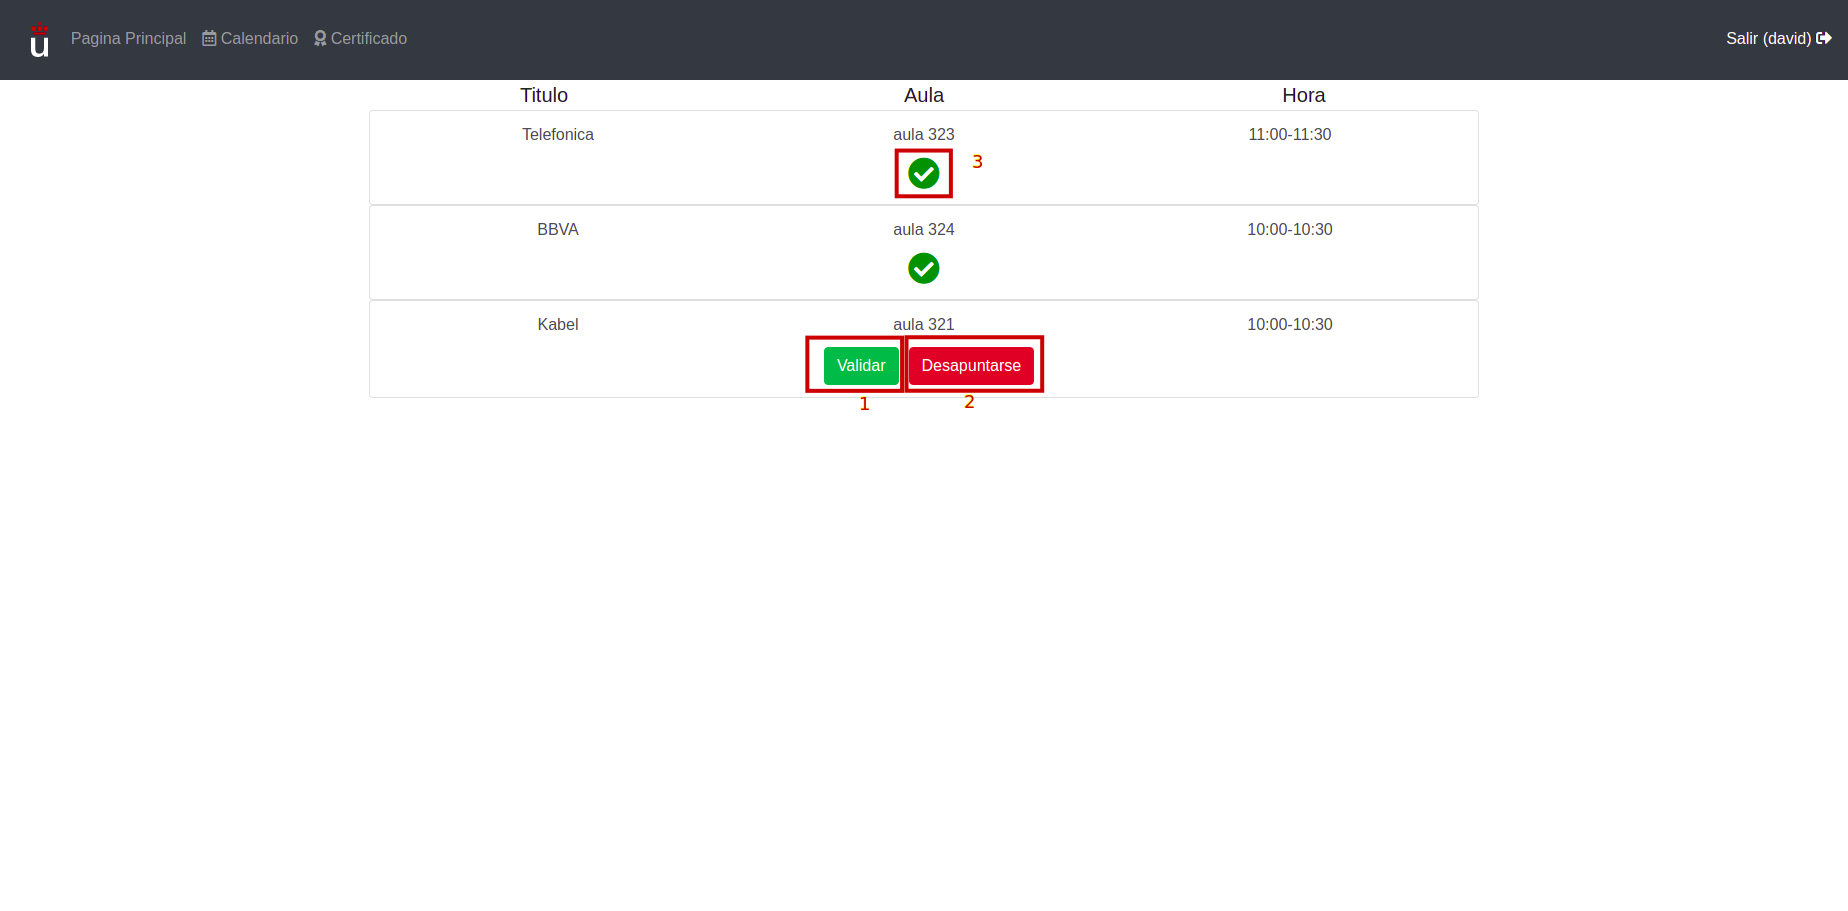
\includegraphics[width=16cm, keepaspectratio]{img/inicio.png}
  	\caption{Página de inicio.}\label{fig:inicio}
	\end{figure}
	
	Una vez presionemos el botón de validar ya que hemos asistido al evento en cuestión y queremos dar fe de ello, la aplicación nos llevará a la pestaña de validación, figura~\ref{fig:validarQR}
	En esta pestaña, la aplicación utilizará la cámara del dispositivo, ya sea un móvil, tabley u ordenador portatil para leer el código QR correspondiente al evento que queremos validar.
	\begin{figure}
  	\centering
  	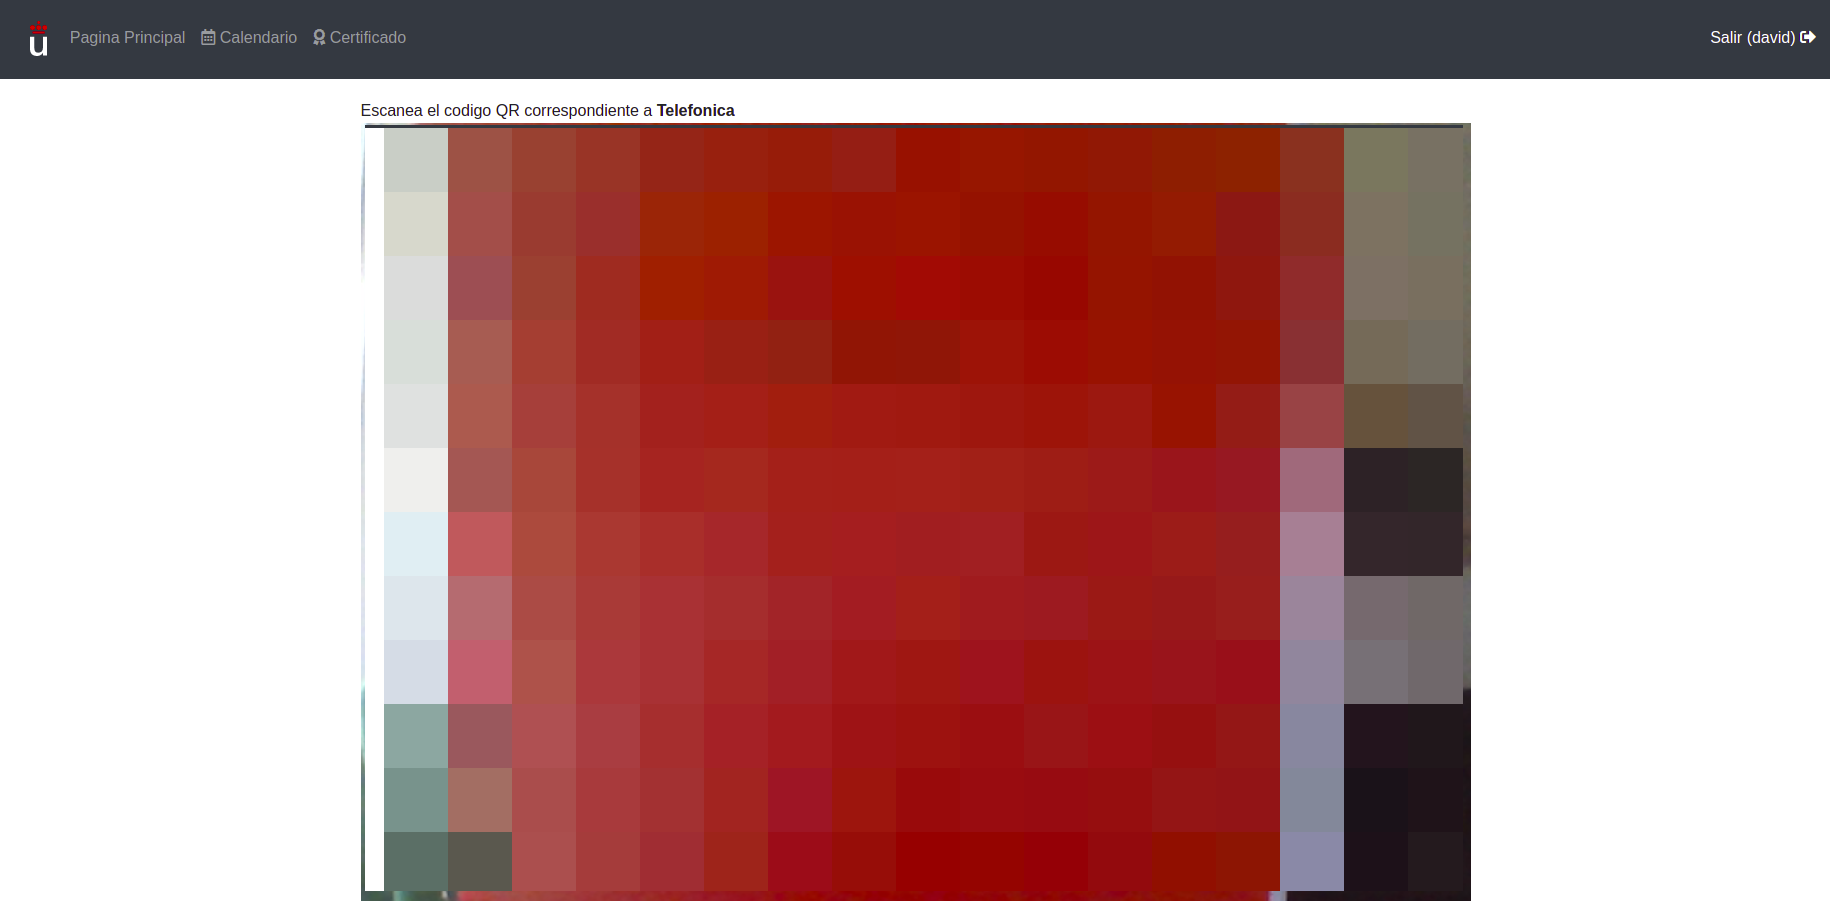
\includegraphics[width=16cm, keepaspectratio]{img/validarQR.png}
  	\caption{Pestaña de validación de QR}\label{fig:validarQR}
	\end{figure}

Para validar el evento, basta con mostrar un QR valido y la aplicación obtendrá un mensaje de aceptación por parte del servidor, si por el contrario mostramos un QR que no correspondería al QR del evento en cuestión, se nos avisará con un mensaje en la pantalla que el QR proporcionado no es válido. En este caso figura~\ref{fig:validarQRFail}, escaneamos un QR correspondiente al evento del BBVA cuando debería ser el QR del evento Telefónica.

	\begin{figure}
  	\centering
  	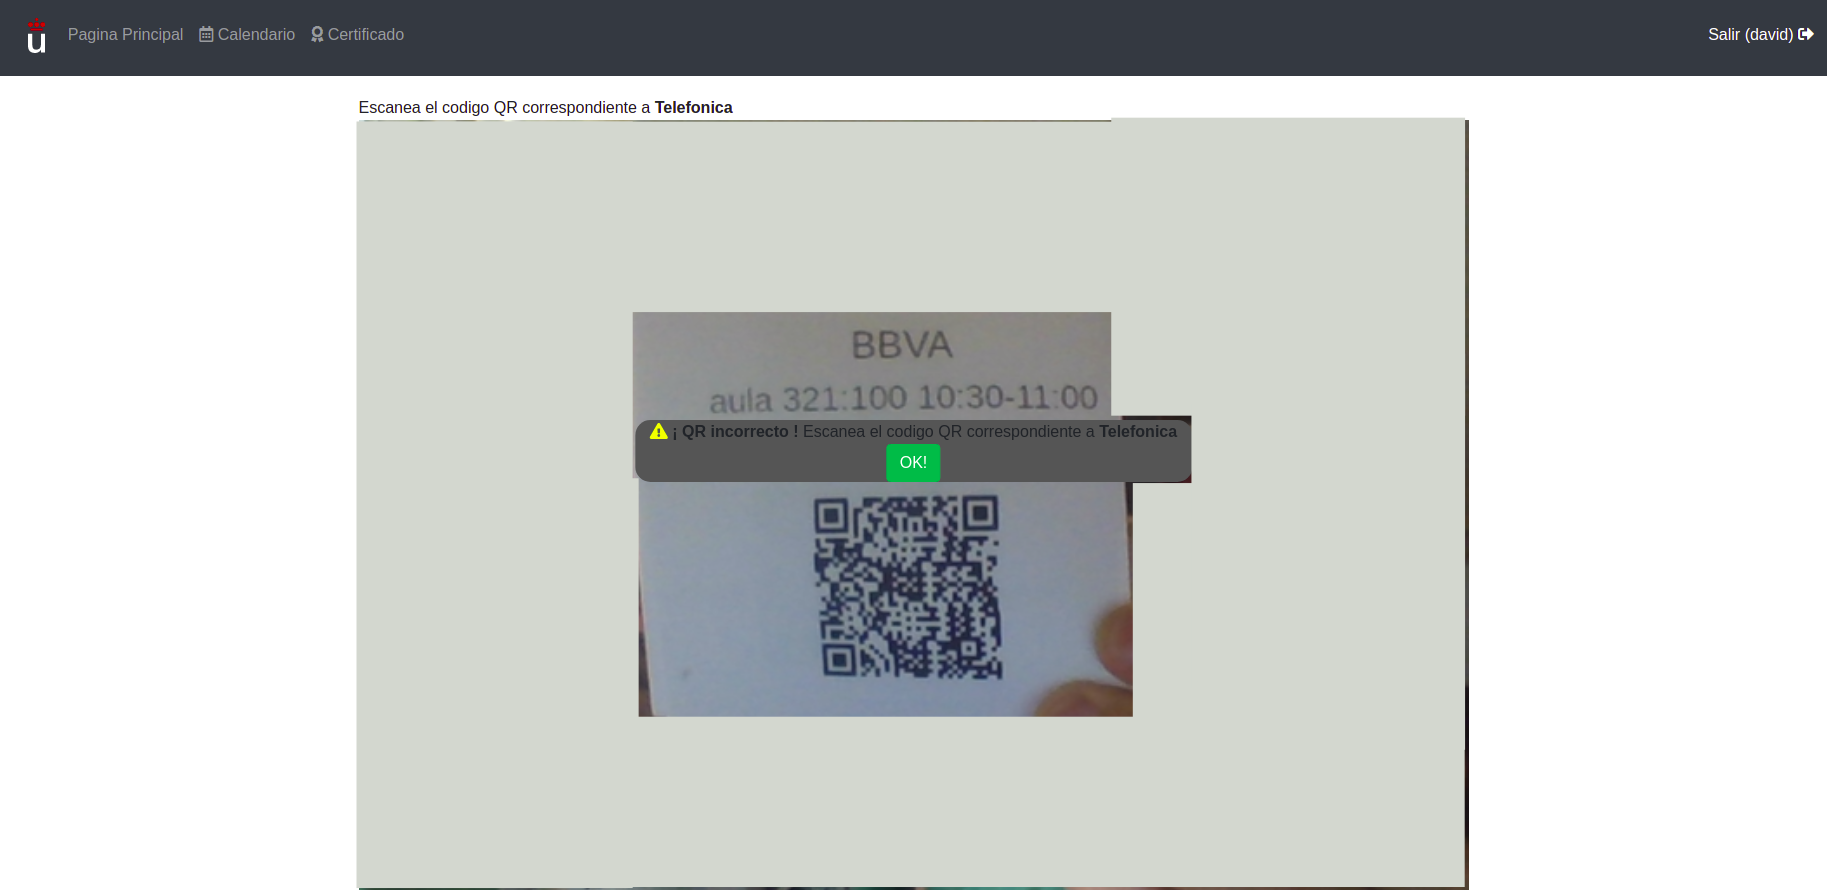
\includegraphics[width=16cm, keepaspectratio]{img/validarQRFail.png}
  	\caption{Pestaña de validación de QR con mensaje de error}\label{fig:validarQRFail}
	\end{figure}  
  
  \item Calendario: En la vista siguiente~\ref{fig:horario} obtenemos un calendario con las principales charlas y seminarios disponibles durante las jornadas habilitadas por la Universidad Rey Juan Carlos. 

\begin{figure}
  	\centering
  	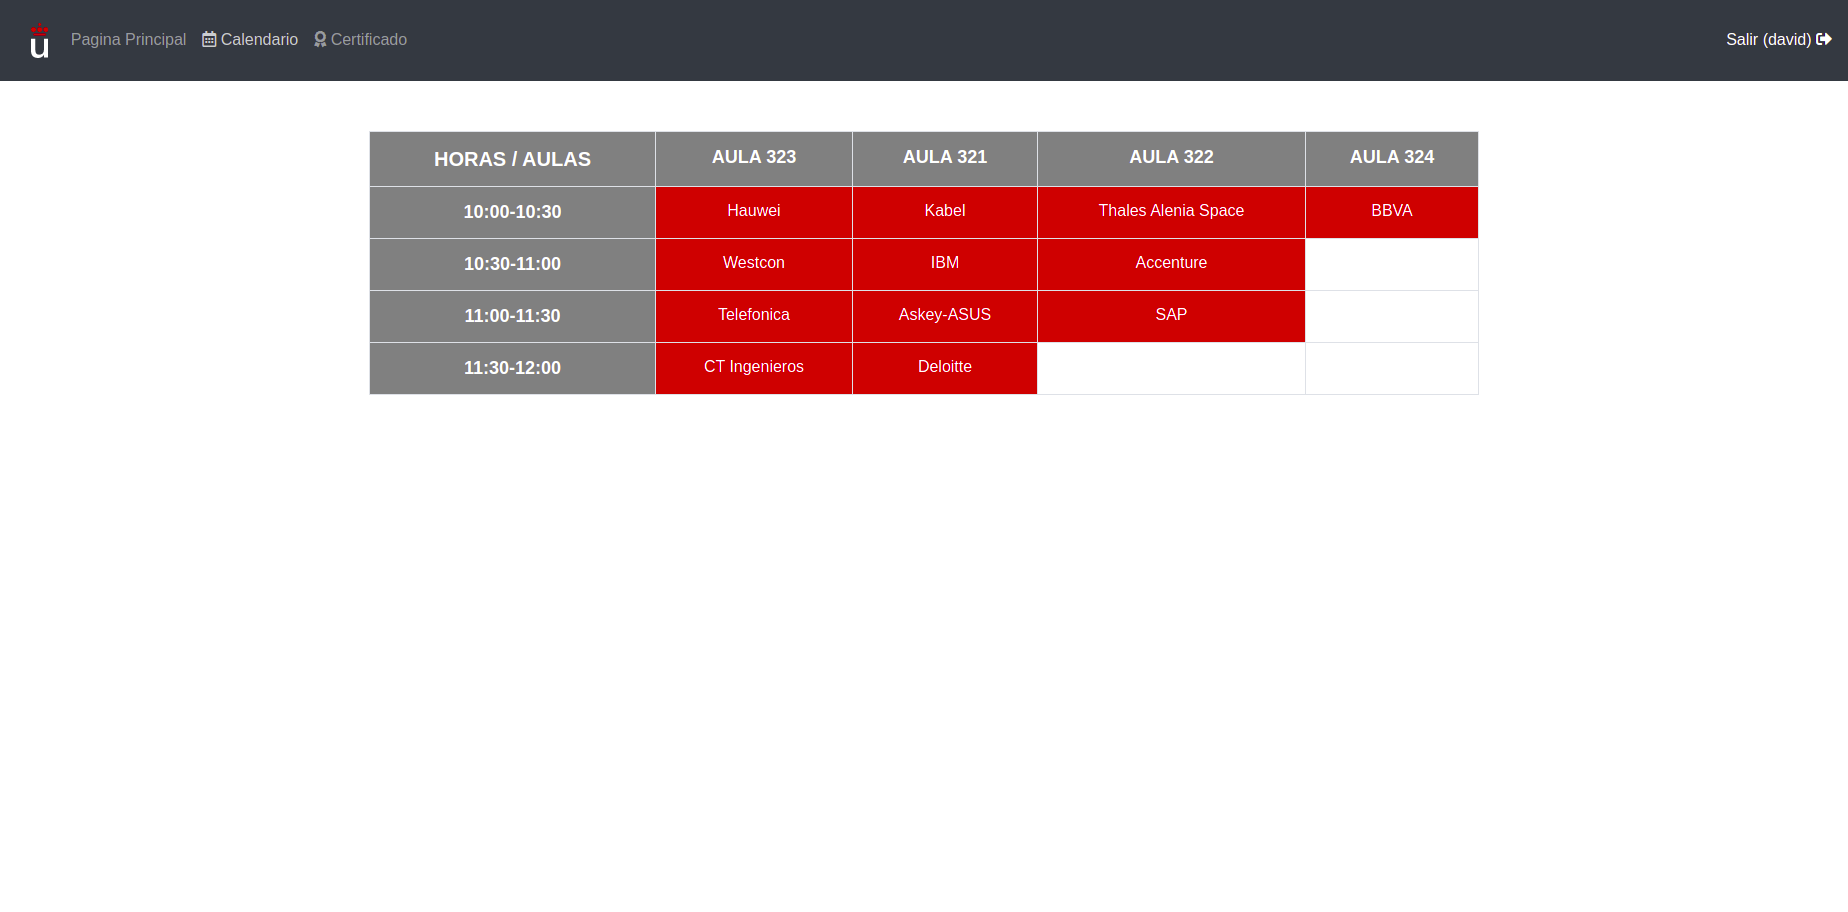
\includegraphics[width=16cm, keepaspectratio]{img/horario.png}
  	\caption{Página de calendario}\label{fig:horario}
	\end{figure}
  
  Cada evento ocupa una posición en el calendario, así mismo cada uno de ellos actúa como un botón, en el que presionándolo nos redirige a la pagina de información del mismo, figura~\ref{fig:descripEvento}. En esta página de información es donde el alumno se podrá apuntarse, dando click en ``Apuntarse'' y expresar su intención de asistir a él, también hay una pequeña descripción del evento que estamos viendo.
  
  \begin{figure}
  	\centering
  	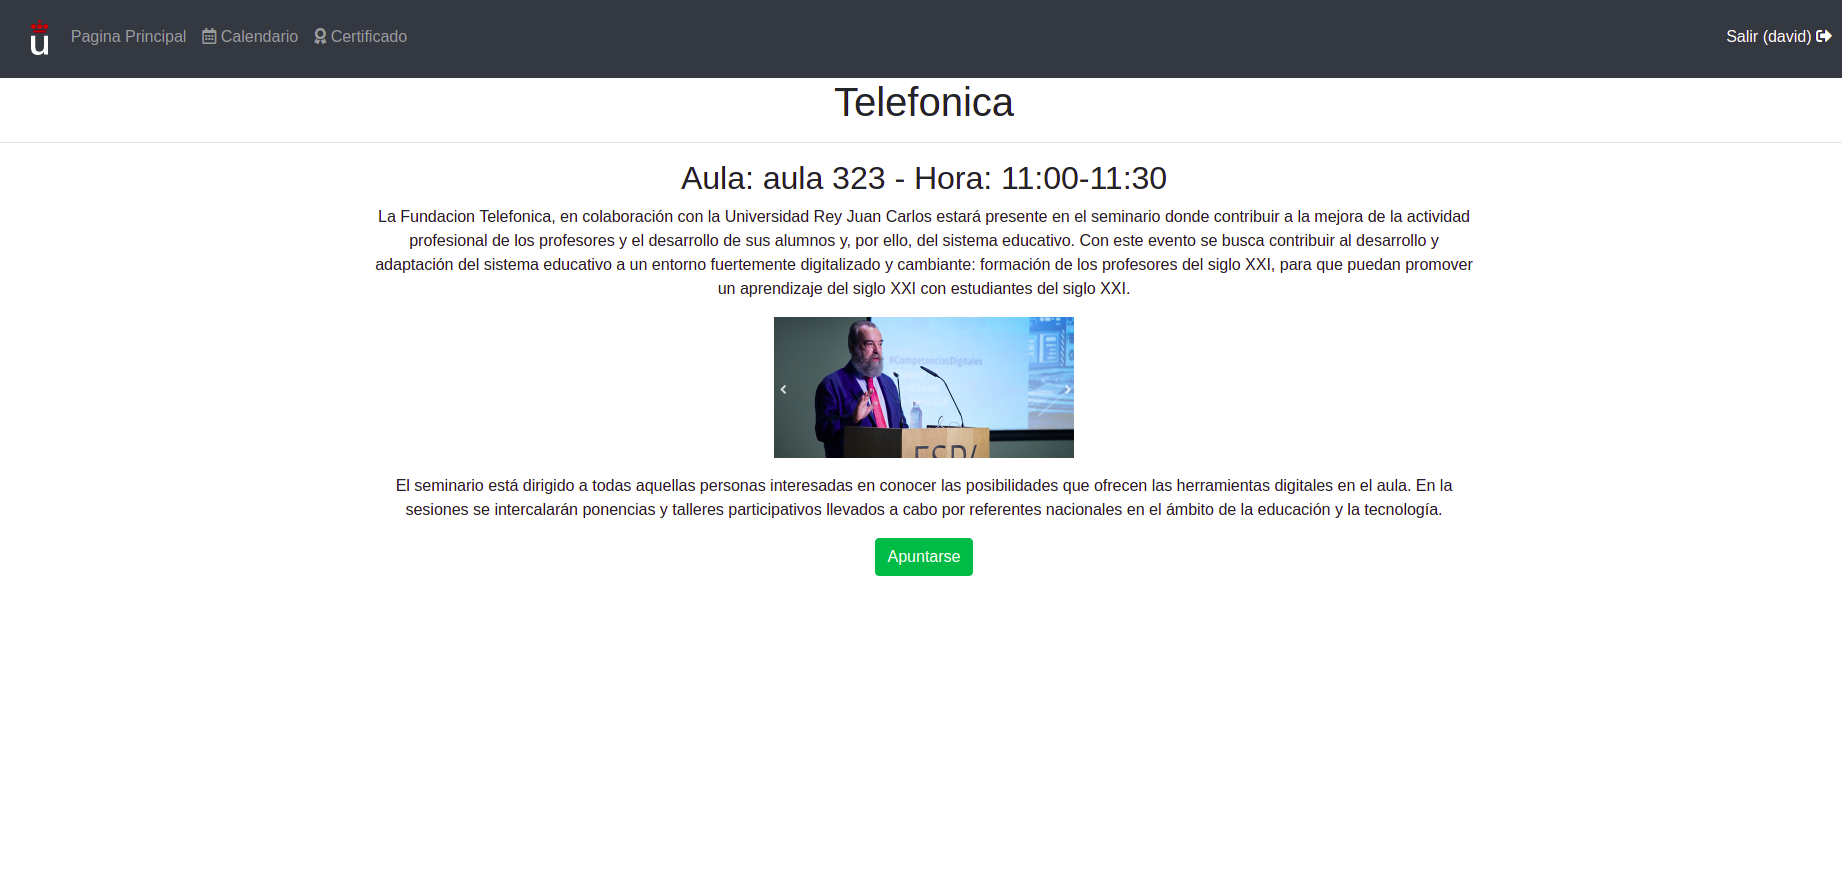
\includegraphics[width=16cm, keepaspectratio]{img/descripEvento.png}
  	\caption{Página de descripción del evento y botón de apuntarse}\label{fig:descripEvento}
	\end{figure}
  
  \item Certificado: Esta vista, figura~\ref{fig:recibirCred}, se compone de un botón que el alumno tendrá disponible únicamente cuando pueda tener la posibilidad de obtener los créditos que le corresponden por asistir a estos seminarios, el requisito de mínimo de asistencia para poder optar a tener el certificado de los créditos lo impondrá el profesor encargado de ello o en su defecto el administrador que se encargue del mantenimiento de la página y de dichas jornadas propuestas aquí. 
  
    \begin{figure}
  	\centering
  	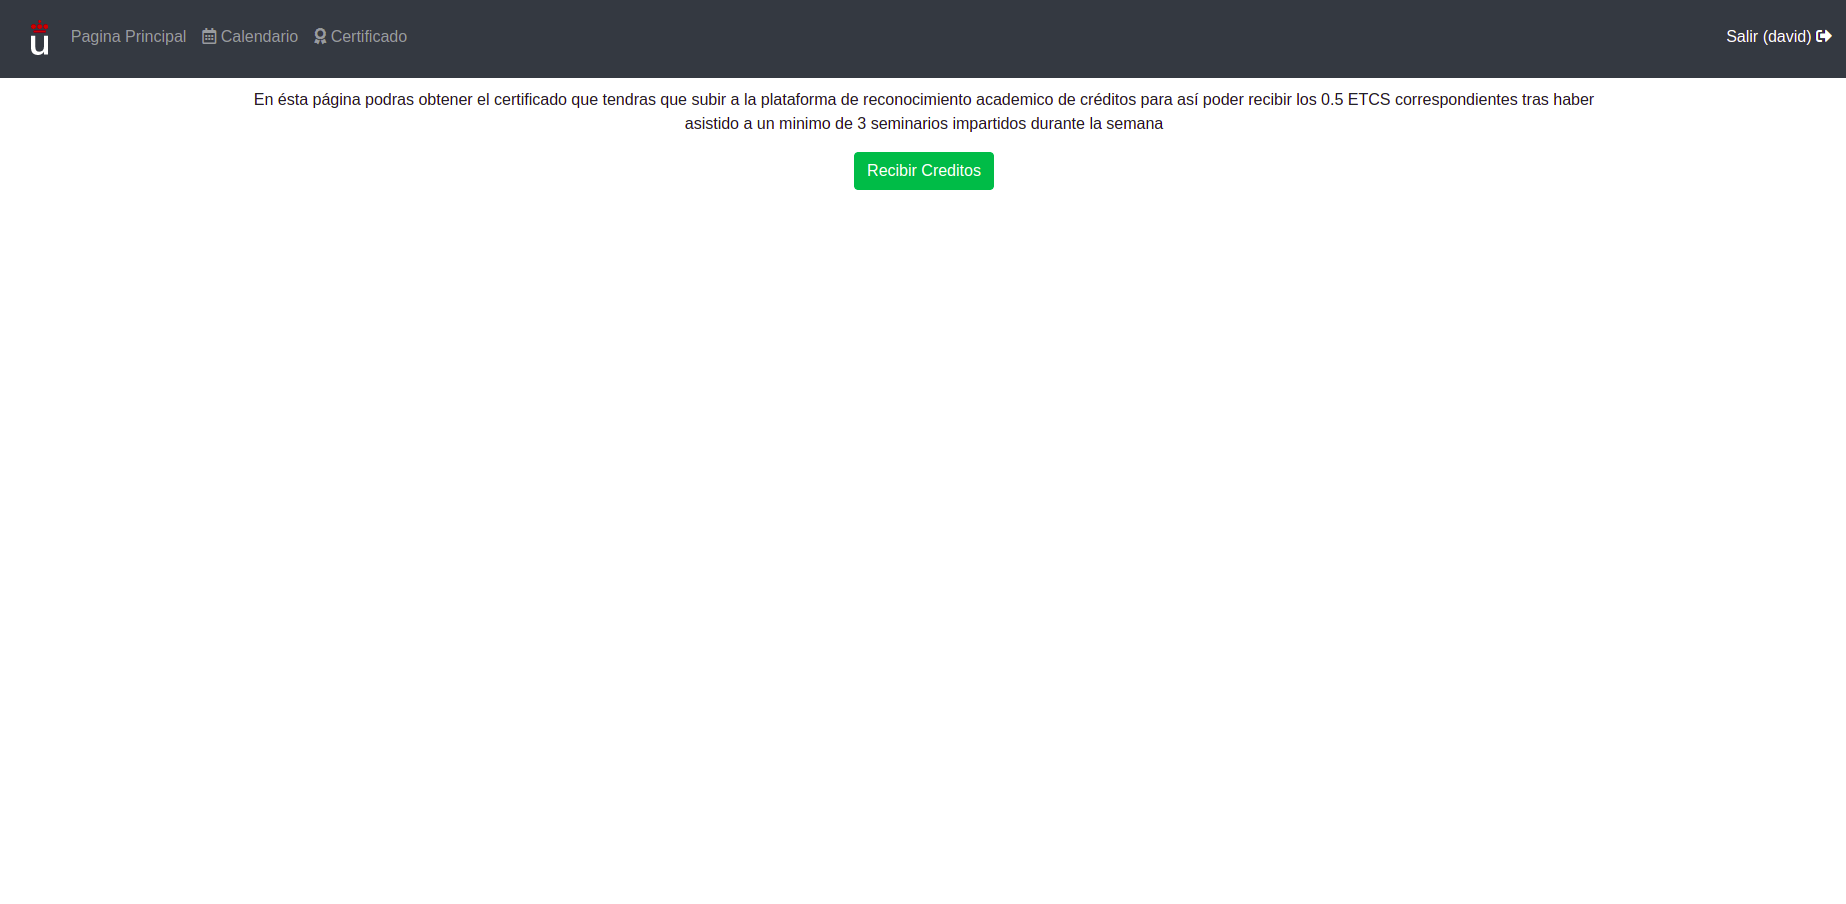
\includegraphics[width=16cm, keepaspectratio]{img/recibirCred.png}
  	\caption{Página para obtener el certificado de créditos}\label{fig:recibirCred}
	\end{figure}
  
  
  Una vez el alumno tiene disponible el botón de ``Recibir Créditos'' un pop-up saldrá en pantalla sirviendo una vista previa del pdf que será el certificado que le otorgue los créditos y que el alumno obtendrá para poder justificar los mismos, como se puede observar en la figura~\ref{fig:pdfVisual}. Estará a su vez disponible un botón de descarga del pdf para poder almacenarlo en su dispositivo.
  
      \begin{figure}
  	\centering
  	
\includegraphics[width=16cm, keepaspectratio]{img/pdfVisual.png}
  	\caption{Pop-up con la vista del certificado}\label{fig:pdfVisual}
	\end{figure}
  
\end{enumerate}

\subsubsection{Administrador}
	Una vez iniciado sesión con la cuenta del administrador o de la persona encargada de mantener y administrar la aplicación entraremos en la misma donde veremos dos pestañas claramente diferenciadas:
\begin{enumerate}	
	\item Lista de Eventos: En esta pestaña representada en la figura~\ref{fig:adminListaEventos}, el administrador de la aplicación tendra un listado completo de todos los eventos o seminarios que habrá durante la semana o los días que duren cada uno de ellos. En esta primera vista se dará la información de: Nombre del evento, aula donde se impartirá y la hora del día a la que tendrá lugar dicho evento.
	\begin{figure}
  	\centering
  	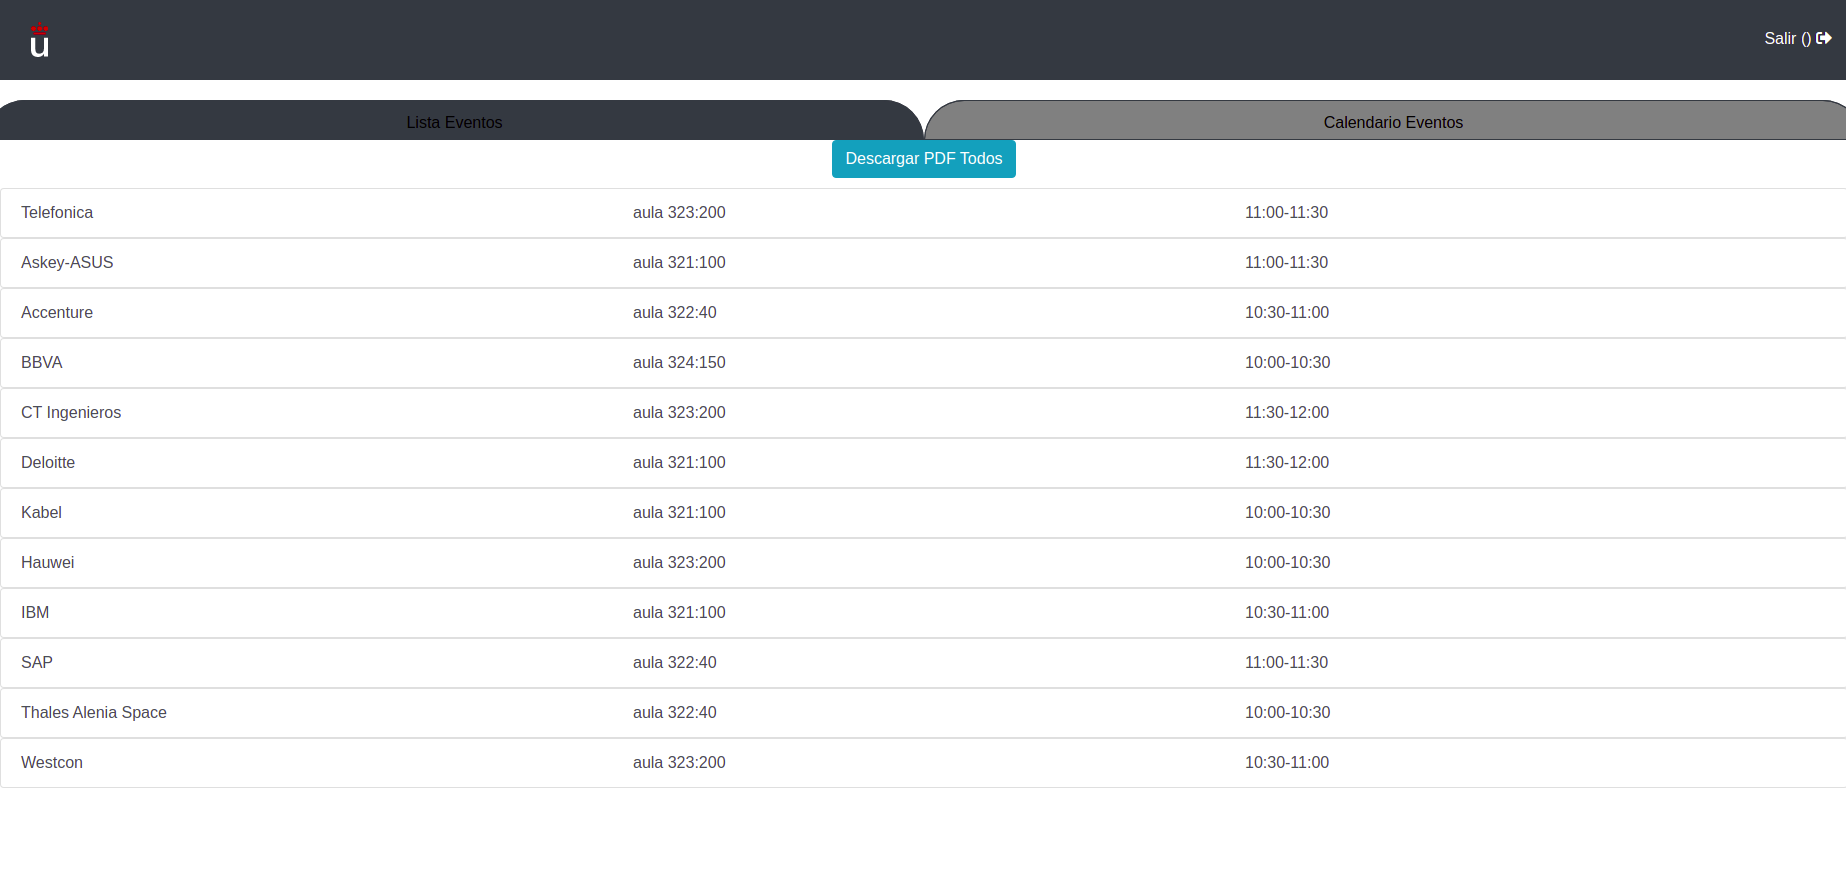
\includegraphics[width=16cm, keepaspectratio]{img/adminListaEventos.png}
  	\caption{Vista de administrador de la pestaña Lista de Eventos}\label{fig:adminListaEventos}
	\end{figure}

Destacamos en esta vista~\ref{fig:AdminEventosZip}, el botón de \textit{``Descargar PDF Todos''}, presionándolo enviaremos una petición al servidor que nos contestará con un archivo comprimido en formato ZIP llamado ``Eventos.zip'' que contendrá todos los CSV de los Eventos en los que haya apuntada mas de una persona. Este CSV es del mismo formato que el CSV que se descargaría dando uno por uno a cada evento con el botón ``Generar CSV'' que explicaremos más adelante en el siguiente punto. El archivo comprimido en formato ZIP descargado quedaría de la siguiente manera:
	
	\begin{figure}
  	\centering
  	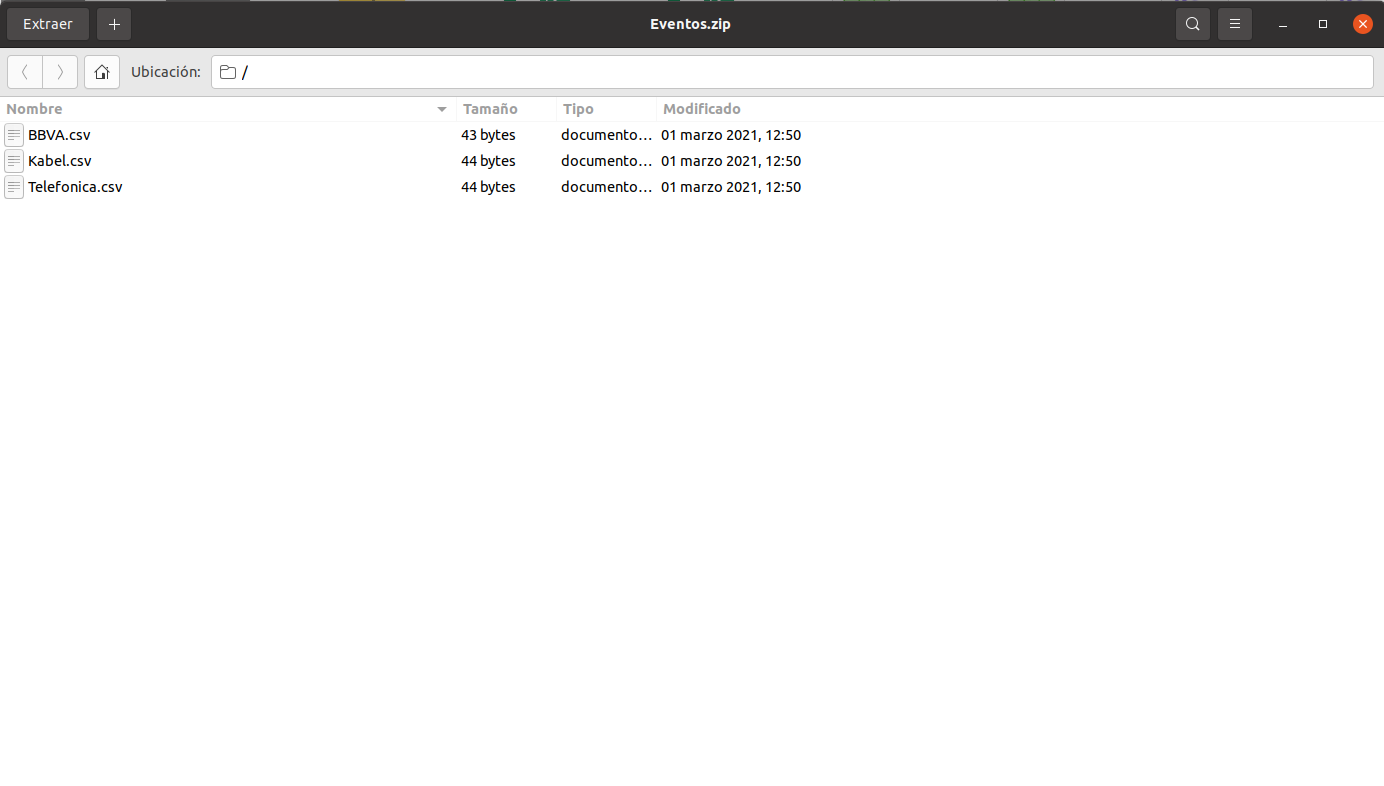
\includegraphics[width=16cm, keepaspectratio]{img/AdminEventosZip.png}
  	\caption{Contenido de Eventos.zip descargado al presionar \textit{Descargar PDF Todos}}\label{fig:AdminEventosZip}
	\end{figure}
	
	 
	Haciendo click en cada una de las filas correspondientes a cada uno de los eventos entraremos en una ventana representada en la figura~\ref{fig:adminListaEventoTelefonica}, donde nos informará más detalladamente sobre el evento en cuestión, con una breve descripción del evento (1), su QR de validación correspondiente (2) y el listado de los usuarios inscritos a él, así como que usuario ha validado o no la asistencia al evento con el campo \textit{``Validado''} true o false (3). Destacamos de esta vista el botón \textit{``Generar CSV''} (4) que descargará en nuestro equipo en formato CSV el mismo listado de usuarios que estamos viendo en esta misma página.
	
	\begin{figure}
  	\centering
  	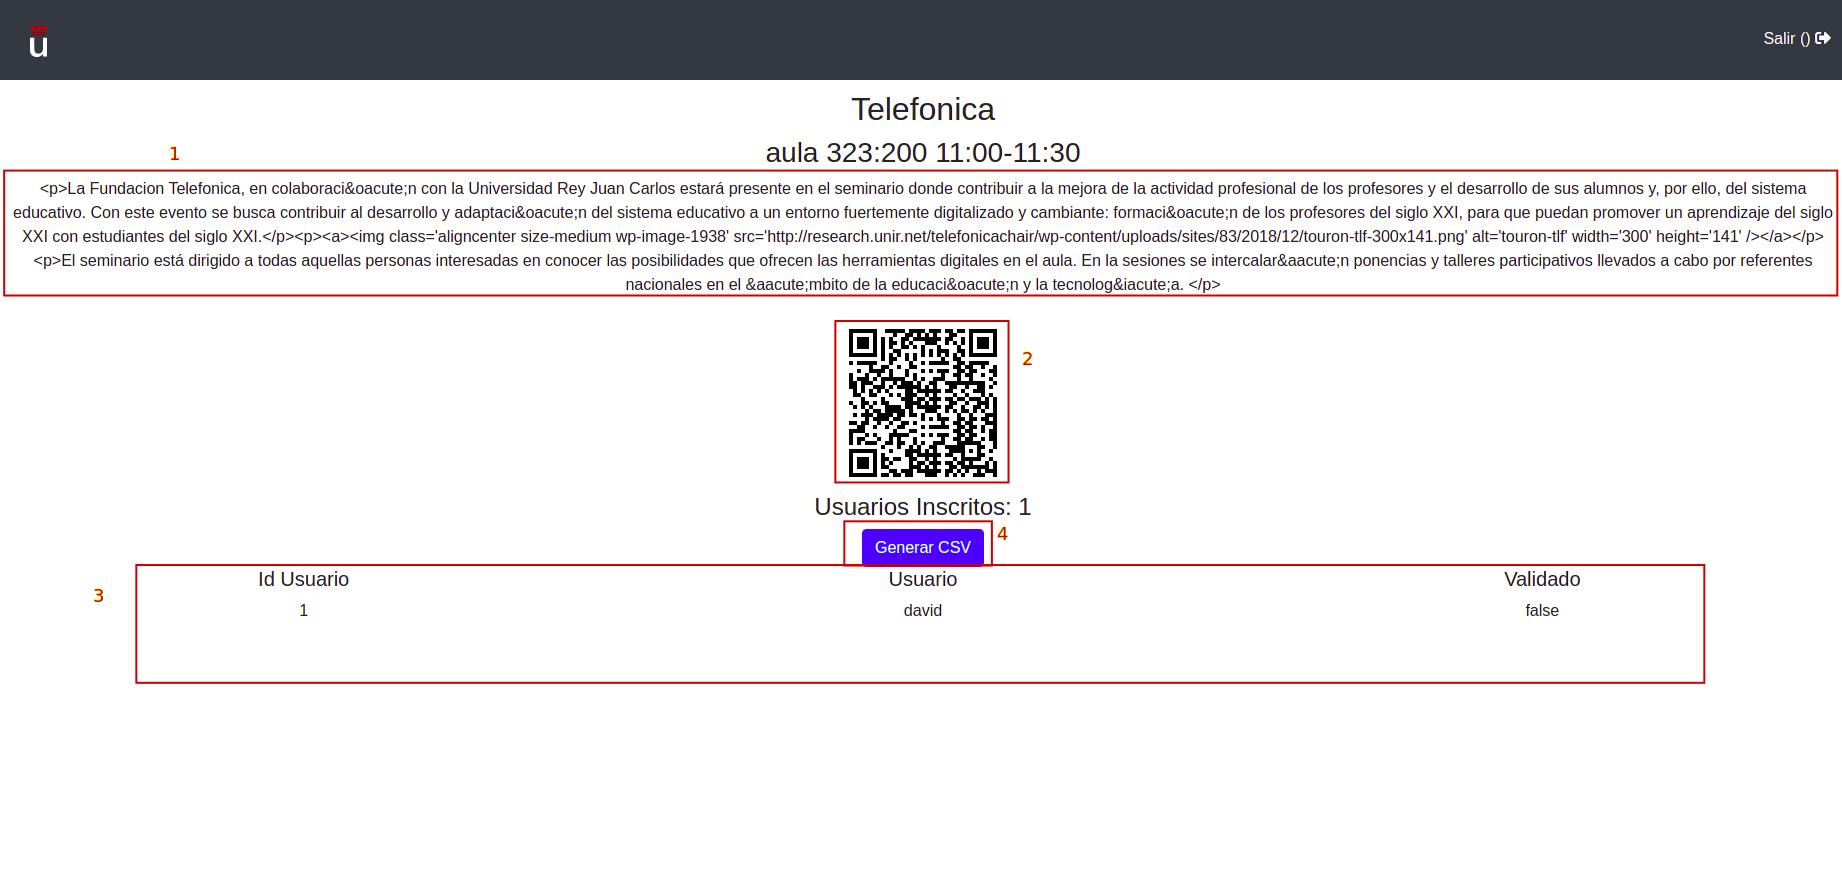
\includegraphics[width=16cm, keepaspectratio]{img/adminListaEventoTelefonica.png}
  	\caption{Vista de administrador de la ventana informativa del evento de Telefónica}\label{fig:adminListaEventoTelefonica}
	\end{figure}


	\item Calendario Eventos: En esta pestaña, figura~\ref{fig:adminCalendario}, el administrador tendrá de forma visual la información de cuando y donde va a tener lugar un evento cualquiera, seguido del nombre del evento, entre paréntesis, hay un número correspondiente al número de alumnos apuntados a dicho evento.
	
	Destacamos varias cosas en esta pestaña, en primer lugar el botón \textit{``Optimizar''}, este botón envía un mensaje al servidor que lanzará un python de optimización para reubicar los eventos en horarios y aulas de la forma lo más óptima posible, más adelante, en el siguiente punto, cuando se explique la parte correspondiente al servidor desarrollaré más su funcionamiento. Este botón modificará la posición de todos o la gran mayoría de los eventos dentro del marco horario mostrado en esta pestaña.
	
	Por otro lado, es posible modificar de forma individual un evento, para ello bastará con hacer click sobre él, toda su información se volcará en los desplegables que se muestran en la parte inferior de la imagen (1), se podrá modificar tanto el aula como las horas que estén disponibles para todos los eventos, en este caso entre las aulas 323, 321, 322 y 324 y en los horarios de 10:00 a 12:00. 
	
	Presionando el botón ``Modificar'' las modificaciones que hayamos hecho en los desplegables serán enviadas al servidor y podremos verlas en esta misma vista.
	
		\begin{figure}
  	\centering
  	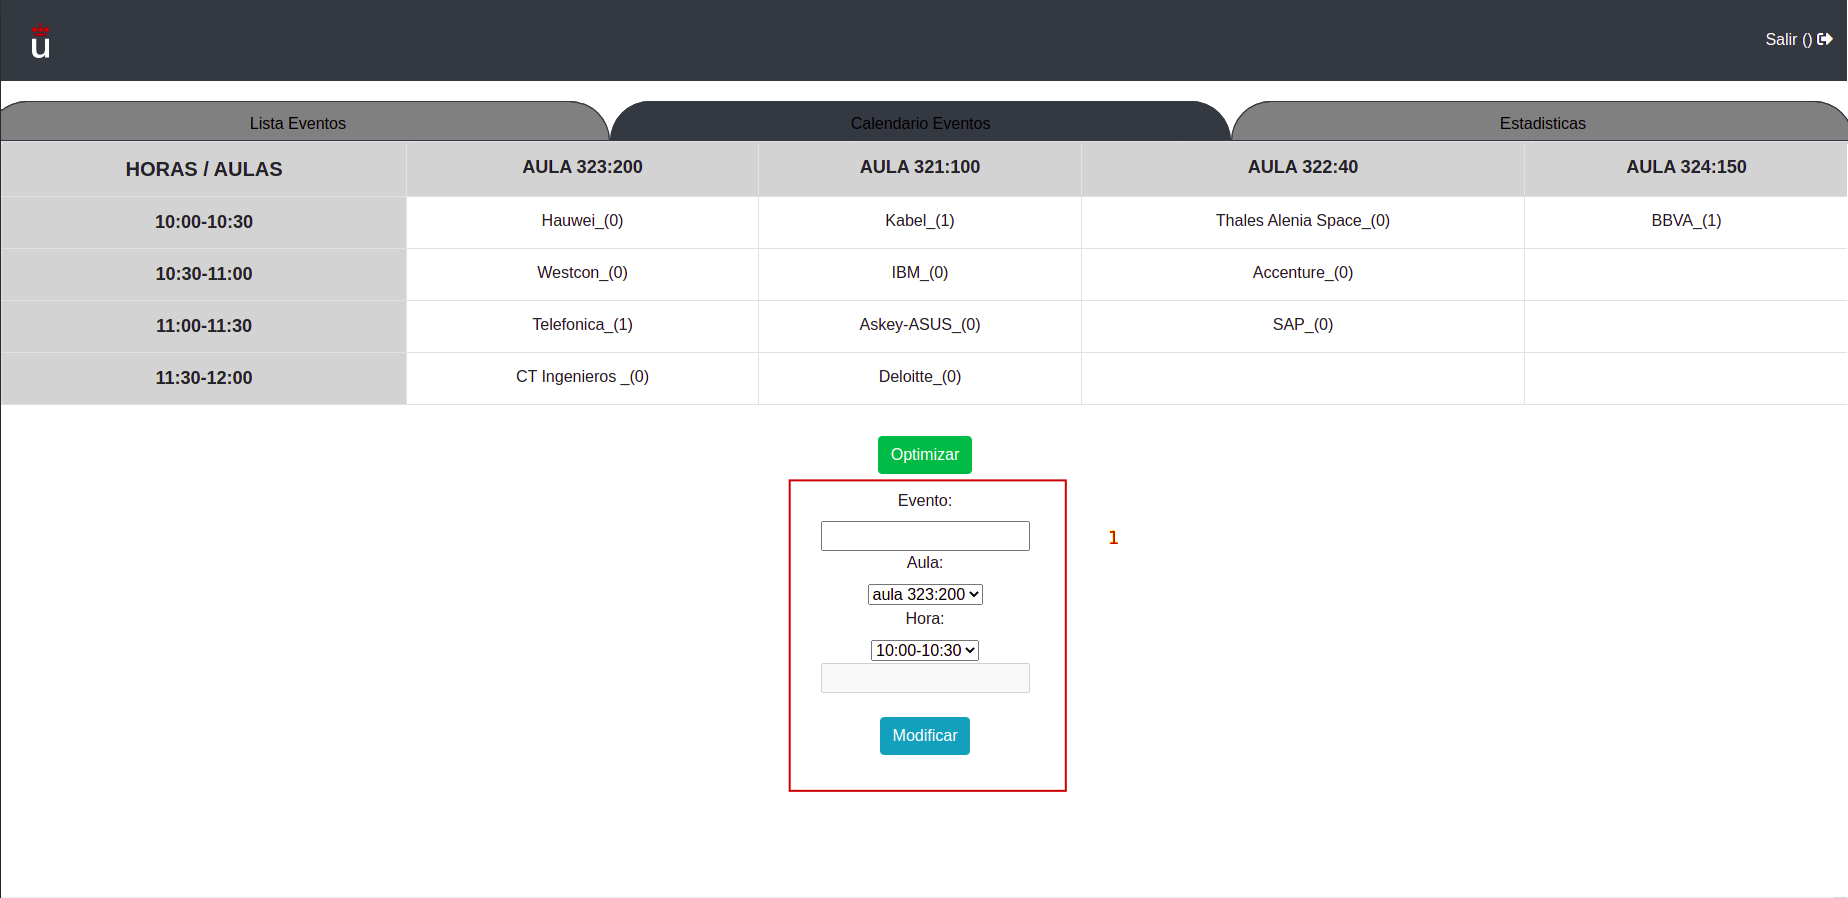
\includegraphics[width=16cm, keepaspectratio]{img/adminCalendario.png}
  	\caption{Pestaña Calendario Eventos}\label{fig:adminCalendario}
	\end{figure}
  
\end{enumerate}

\subsection{Servidor}

	El servidor está desarrollado en un entorno de trabajo que funciona en tiempo de ejecución, de código abierto y multiplataforma, este entorno es \textit{Node}. Añade un soporte para APIs donde se incluye una comunicación HTTP entre el cliente y él mismo. Por todo esto obtenemos un gran rendimiento de la aplicación y también una gran escalabilidad. Dentro de Node el framework mas usado y que uso en este caso es \textbf{Express} cuya librería se compone de un gran número de framework populares dando mecanismos para el manejo de peticiones HTTP y HTTPS (en mi caso) y mantener así una comunicación segura cliente-servidor. 
	Los métodos de comunicación usados en el servidor mediante HTTPS son los típicos usados en este tipo de aplicaciones:
	\begin{itemize}
  	\item GET: El método GET  solicita una representación de un recurso específico. Las peticiones que usan el método GET sólo deben recuperar datos.
  	\item POST: El método POST se utiliza para enviar una entidad a un recurso en específico, causando a menudo un cambio en el estado o efectos secundarios en el servidor.
  	\item PUT: El modo PUT reemplaza todas las representaciones actuales del recurso de destino con la carga útil de la petición.
  	\item DELETE: El método DELETE borra un recurso en específico.
	\end{itemize}

Al margen ya de la parte Node del servidor, destacamos dos programas desarrollados en python de los que el servidor hace uso cuando el cliente así lo requiere, destacamos que el único cliente o usuario que puede realizar una petición al servidor y poder lanzar así estos programas es el usuario bajo el Nick de ``admin'', en los siguientes puntos pasaremos a explicar el funcionamientos de dichos programas:

\begin{enumerate}
  	\item CreateCSV.py: Cuando el administrador presiona dentro de la pestaña ``Lista Eventos'' cualquier fila correspondiente a un evento, y dentro de ella el botón ``GenerarCSV'' o bien en la misma pestaña de ``Lista Eventos'' presiona el botón ``Generar PDF Todos'', el servidor dentro de la url \textit{'/zip/:id\_evento/:nombre\_evento'} recibe la petición del cliente que quiere obtener o bien un CSV o bien un .zip con todos los CSV de los eventos dentro de él. Desde Node se lanza el python mediante el comando ./createCSV.py -idevento (el parametro idevento solo se pondrá en el caso en el que se quiera el CSV de un evento en concreto, para obtener el .zip de todos el parametro se omitirá).
  	
  	Una vez el programa en python de createCSV.py ha sido lanzado, pasa a buscar en la base de datos mediante un select de idevento o recorriendose todos los eventos que haya obteniendo así una lista de usuarios asociados al evento con el campo validado true o false según corresponda para cada uno de los usuarios.
  	
  	Cuando se obtiene esta lista y se finaliza la ejecución del select, pasamos a volcar los datos obtenidos en un fichero .CSV, cuando terminamos de rellenar el fichero, en el caso de querer uno en concreto la ejecución terminaría aquí y sería devuelto el fichero al cliente que solicitó tal acción al servidor, por otro lado, en el caso de querer todos los eventos se irá completando la acción pasada con todos los eventos en los que haya mas de una persona inscrita en él, y cuando termine pasaŕa a crear un .zip con todos estos .CSV creados. Una vez terminado, como en el caso anterior, le será devuelto al cliente un .zip como requirió con su petición inicial.
  	
  	La forma en la que el servidor y el cliente están conectados para poder enviar la información en formato .CSV o en formato .ZIP es mediante un \textit{pipe stream.}
  	
  	La funcionalidad y el esquema de dicho funcionamiento quedan representadas en la figura~\ref{fig:createCSV}.

\begin{figure}
  \centering
  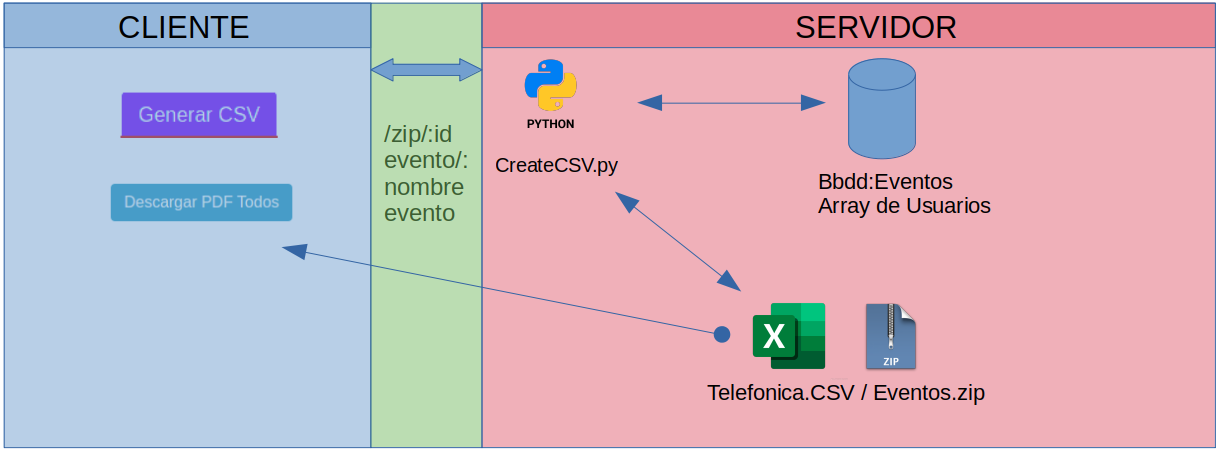
\includegraphics[width=16cm, keepaspectratio]{img/createCSV.png}
  	\caption{Esquema funcionamiento createCSV.py}\label{fig:createCSV}
\end{figure}  	
  	
  	
  	\item optimizarSalas.py: El siguiente programa se ejecuta cuando el administrador dentro de la pestaña ``Calendario Eventos'' presiona el botón ``Optimizar'', este botón lanza un mensaje a la ruta \textit{'/optimizar'} dentro el endpoint donde está escuchando el servidor, que ejecuta el comando \textit{'./optimizarSalas.py'} lanzando el programa en python. 
  	
  	Este programa tiene como objetivo la optimización y reubicación de los eventos en función de los huecos libres que quedan con respecto a la gente que se ha apuntado al evento o quiere asistir y con los huecos libres que quedan en la sala. Funciona de la siguiente manera:
  	
  	El programa, una vez se ejecuta, lee de la base de datos cada uno de los eventos que están programados que se van a llevar a cabo en los días que transcurran todos ellos, de cada evento obtiene el número de alumnos o personas que están apuntados a él, con este número calcula los huecos libres que tienen en todas las aulas disponibles, desechando los números negativos que se obtienen cuando van a asistir mas personas que huecos libres tiene la sala.
  	
  	Una vez tenemos relacionados todos los eventos con las aulas en función de los huecos libres que hay, el diccionario se ordena de menor a mayor, teniendo prioridad de posición los eventos que tengan menor número de huecos libres en una sala determinada.
  	 
  	La adjudicación del evento a una sala se va realizando de forma ascendente y ordenada hasta que el aula en cuestión complete todas las horas disponibles que tiene dentro de los días que están programados que tengan lugar estos eventos. En nuestro caso, se completara cuando en una sala se haya completado el horario de 10:00 a 12:00, cuando esto ocurre el evento no tendrá la opción de ser colocado en esa aula y pasará a ka siguiente aula donde en función del tamaño, las personas que vayan y el número de huecos disponibles sea el óptimo.
  	
  	Si se llega a el caso en el que un evento no encuentra lugar dentro de ningún aula, este evento quedará excluido y no se le adjudicará ningún aula. El evento se mostrara fuera de la matriz de ``Calendario Eventos''  y tendrá que ser el administrador quien lo posicione a mano, dentro de un aula en concreto teniendo en cuenta la limitación de aforo mediante el botón ``Modificar'' que se encuentra en la parte inferior de la pestaña de ``Calendario Eventos'' y que ya explicamos su funcionamiento en el apartado anterior.
	\end{enumerate}

%%%%%%%%%%%%%%%%%%%%%%%%%%%%%%%%%%%%%%%%%%%%%%%%%%%%%%%%%%%%%%%%%%%%%%%%%%%%%%%%
%%%%%%%%%%%%%%%%%%%%%%%%%%%%%%%%%%%%%%%%%%%%%%%%%%%%%%%%%%%%%%%%%%%%%%%%%%%%%%%%
% EXPERIMENTOS Y VALIDACIÓN %
%%%%%%%%%%%%%%%%%%%%%%%%%%%%%%%%%%%%%%%%%%%%%%%%%%%%%%%%%%%%%%%%%%%%%%%%%%%%%%%%

\cleardoublepage
\chapter{Pruebas y funcionamiento}

El principal objetivo sobre el que gira este proyecto de fin de grado es el de crear una aplicación web híbrida que funcione tanto en dispositivos móviles como en navegadores web, esto lo hemos conseguido creando una Aplicación Web Progresiva o PWA. 

Para ver que realmente hemos conseguido que nuestra aplicación sea una PWA basta con realizar las siguientes pruebas: 

\section{Server Workers}
Nuestra aplicación contiene \textit{server workers} que son propios del paquete \textit{@angular/pwa v.0.1101.1} para ello basta con mirar en la consola de desarrolladores de Google Chrome o de cualquier navegador, ir al apartado service workers y ver que está activado y corriendo como observamos en la figura~\ref{fig:serviceWorker}
	
	\begin{figure}
  	\centering
  	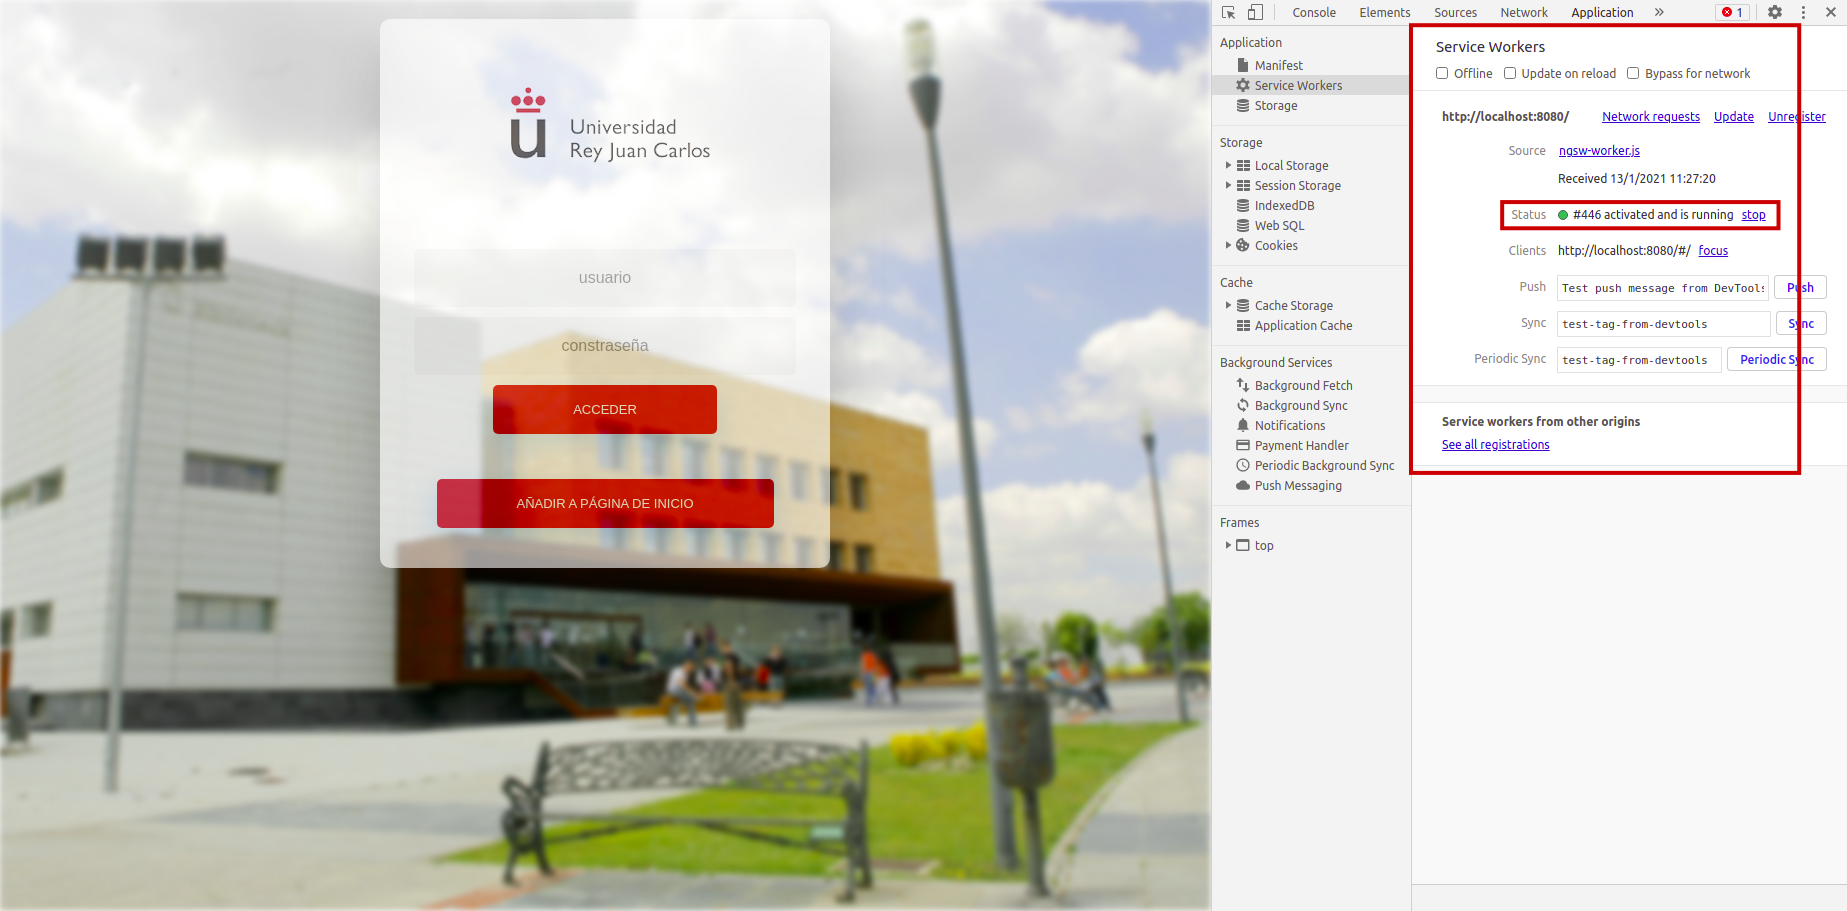
\includegraphics[width=16cm, keepaspectratio]{img/principalWorker.png}
  	\caption{Service Workers funcionando en la PWA}\label{fig:serviceWorker}
	\end{figure}
	  
\section{Instalación en un dispositivo móvil}
Podemos instalar nuestra aplicación en un dispositivo móvil como si de una aplicación nativa, android o IOS, se tratase. Para ello presionamos el botón ``Añadir a pagina de inicio'' una vez que estemos navegando con el dispositivo móvil en cuestión por nuestra aplicación.
	Una vez hayamos aceptado y se haya instalado, nuestra aplicación PWA se verá como una aplicación nativa dentro de nuestro dispositivo móvil como podemos observar en la figura~\ref{fig:homeMovil} 
 
	\begin{figure}
  	\centering
  	
\includegraphics[width=5cm, keepaspectratio]{img/addHomeMovil.png}
  	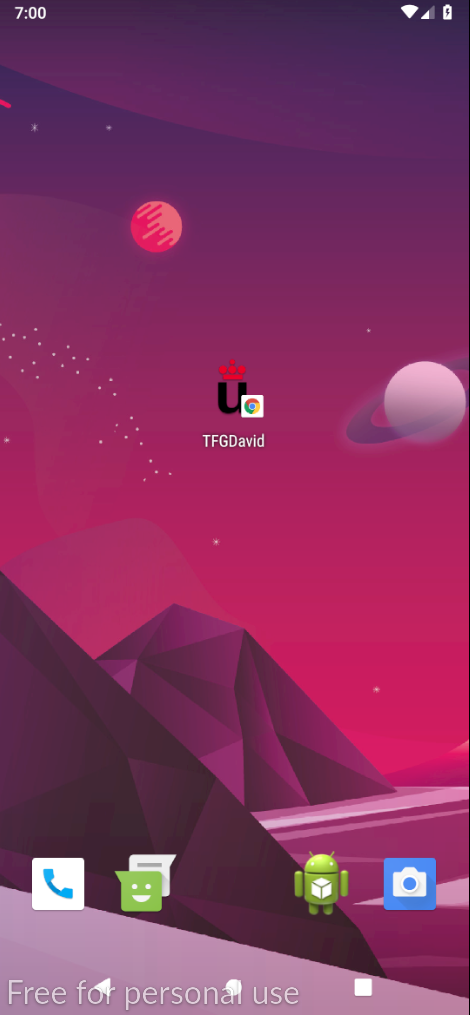
\includegraphics[width=5cm, keepaspectratio]{img/homeMovil.png}
  	\caption{PWA en la pantalla de inicio del dispositivo móvil}\label{fig:homeMovil}
	\end{figure} 
 
\section{Optimización}
En cuanto a la parte del servidor, un punto importante a tener en cuenta sobre la validación del proyecto y el buen funcionamiento de este es que el python encargado de optimizar las salas en función al número de alumnos apuntados y al número de huecos disponibles funcione correctamente. Para ello podemos lanzar manualmente el propio python encargado de ello con el comando \textit{python optimizarSalas.py} obtendríamos un resultado como vemos a continuación en la figura~\ref{fig:terminalOptimizar}:
 
 \begin{figure}
  	\centering
  	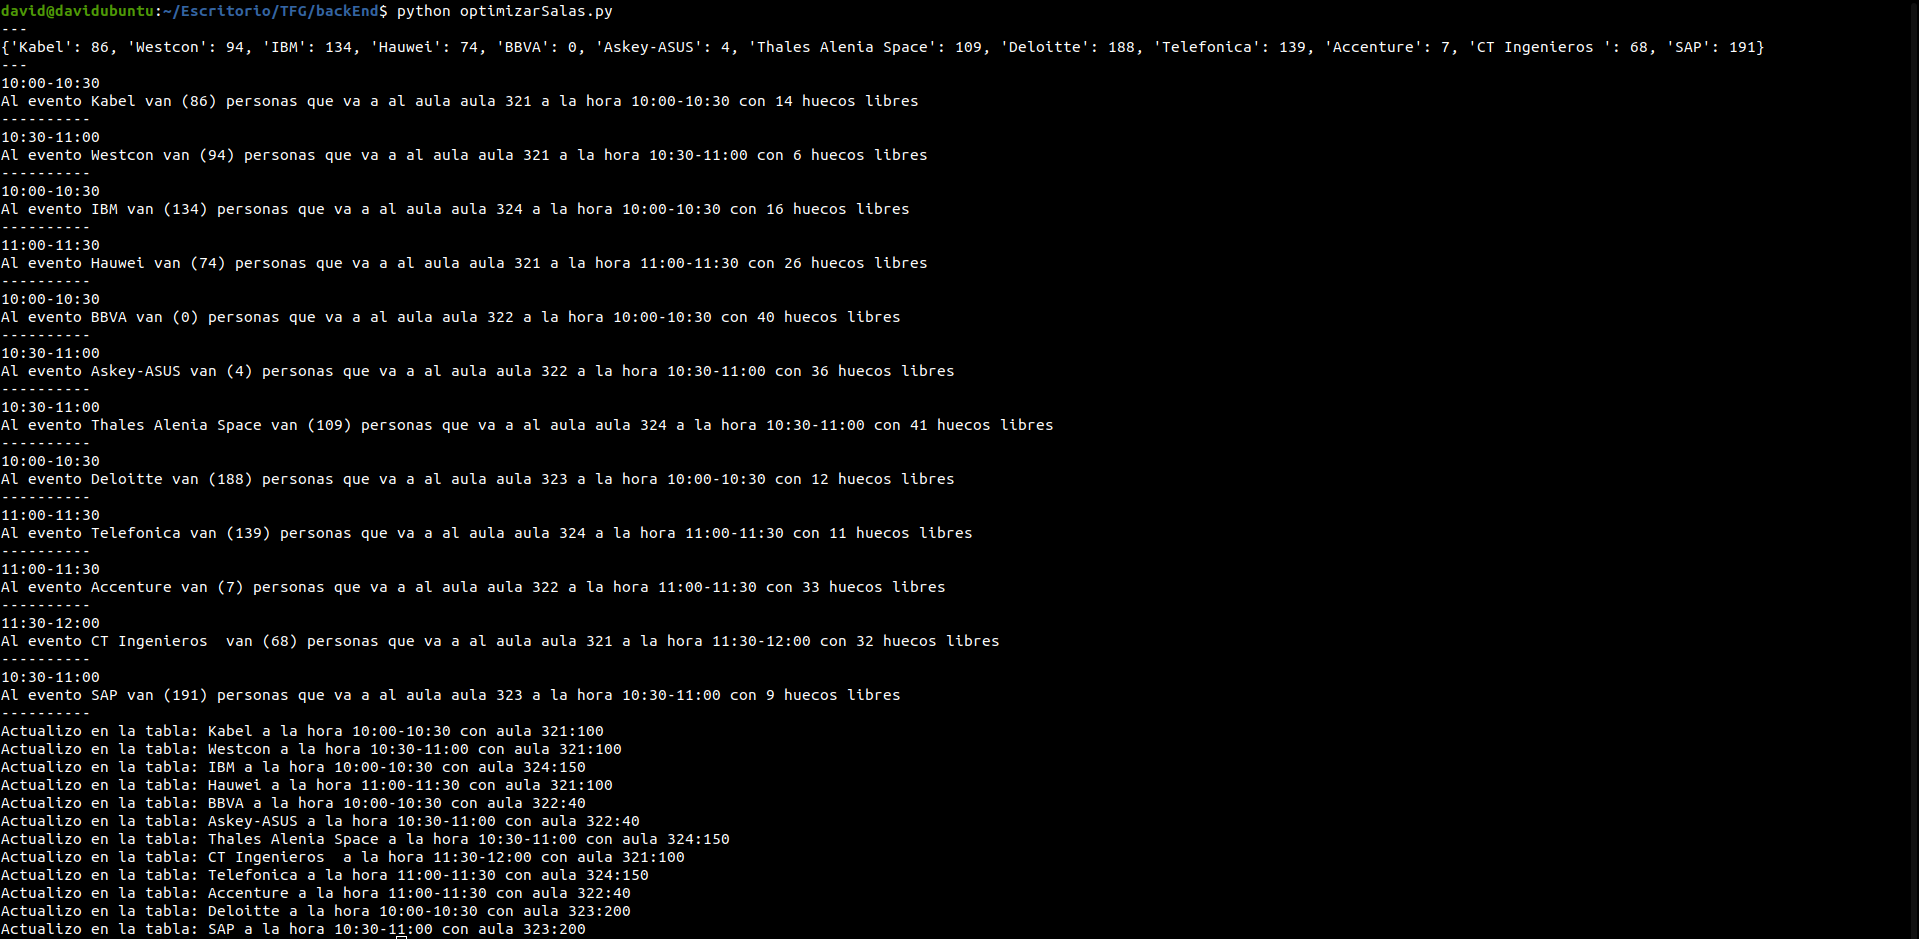
\includegraphics[width=16cm, keepaspectratio]{img/terminalOptimizar.png}
  	\caption{Salida tras ejecutar python optimizarSalas.py}\label{fig:terminalOptimizar}
	\end{figure}
 
Revisando dichos resultados nos damos cuenta que el programa tiene en cuenta los huecos libres de las aulas, el tamaño de la misma y los usuarios inscritos optimizando su distribución.


\section{Seguridad}
Cabe destacar el uso de HTTPS, (HyperText Transfer Protocol Secure, Protocolo de transferencia de hipertexto) es un protocolo de comunicación de Internet que protege la integridad y la confidencialidad de los datos de los usuarios entre sus ordenadores y el sitio web. En este caso al usar partes vulnerables del móvil, como puede se la cámara al leer el código QR o en el momento de autentificar al usuario, es necesario el uso de una capa más de seguridad.
 
 
En el caso de la autenticación la contraseña del usuario, viaja cifrada dentro de este protocolo y dentro de la base de datos permanece cifrada también por si esta base de datos sufre un ataque no se vea comprometida la seguridad de los usuarios de la aplicación.
El cifrado de la contraseña es del tipo \textit{AES192} (Advanced Encryption Standard) y para validar este cifrado basta con ver la base de datos y el valor del campo ``password'' dentro de la tabla ``Usuarios'', en este caso para el usuario \textit{david} el valor del campo es: \textit{4232a5e307a998a3ef2601c7d0a4c704}, un valor esperado para este tipo de cifrados.



%%%%%%%%%%%%%%%%%%%%%%%%%%%%%%%%%%%%%%%%%%%%%%%%%%%%%%%%%%%%%%%%%%%%%%%%%%%%%%%%
%%%%%%%%%%%%%%%%%%%%%%%%%%%%%%%%%%%%%%%%%%%%%%%%%%%%%%%%%%%%%%%%%%%%%%%%%%%%%%%%
% RESULTADOS %
%%%%%%%%%%%%%%%%%%%%%%%%%%%%%%%%%%%%%%%%%%%%%%%%%%%%%%%%%%%%%%%%%%%%%%%%%%%%%%%%

\cleardoublepage
\chapter{Resultados}

El presente proyecto pretendía ofrecer una herramienta de gestión y administración de los eventos o seminarios que se ofrecerán durante la semana cultural, una semana donde los alumnos tienen la oportunidad de interactuar con las distintas empresas del sector en el que están desarrollando su formación universitaria.

La aplicación desarrollada en este proyecto pretende abordar y resolver los objetivos descritos en el punto 2, donde hemos obtenido los siguientes resultados:

\begin{itemize}
  \item Hemos conseguido, mediante un script desarrollado en python, automatizar el proceso de reparto de las clases/horas para las distintas charlas y seminarios en función de los alumnos que se apuntaron a ellas. Este era un objetivo primordial cuando se abordó este TFG, ya que con la automaticación de este proceso le quitamos mucha carga de trabajo al encargado de tal función, en este caso un docente de la universidad.
  
  \item La aplicación está capacitada para crear informes, mediante archivos csv, sobre los alumnos que se han apuntado y han asistido a cada una de las charlas, estos informes serán muy valiosos tanto para la universidad como para las propias empresas que impartirán estas charlas para asi poder enforcarlas en una determinada dirección logrando asi llamar más la atención de los alumnos y conseguir levantar un interés mayor en ellos.
   
   \item Para los alumnos: se ha implementado una aplicación de fácil manejo, muy accesible y que permite mantener informado al alumno en todo momento del horario, tipo de charla que se impartirá y el contenido de la misma. También facilita y agiliza el proceso de verificaciñon de la asistencia a a cada una de ellas y por consiguiente, adquirir los créditos correspondientes.
   
   \item En cuanto a las tecnelogías usadas, se demuestra que disponemos de herramientas muy potentes para poder desarrollar aplicaciones hibridas, que no son muy conocidas actualmente, pero que en un futuro podrán imponerse frente a las aplicaciones nativas. Con este tipo de desarrollos se podrá optimizar el tiempo que conlleva crear una aplicación de este tipo, reduciendo el número de personal necesario para abarcar un mayor público y tener un mayor abanico de posibilidades a la hora de orientar tu aplicación.
\end{itemize}


%%%%%%%%%%%%%%%%%%%%%%%%%%%%%%%%%%%%%%%%%%%%%%%%%%%%%%%%%%%%%%%%%%%%%%%%%%%%%%%%
%%%%%%%%%%%%%%%%%%%%%%%%%%%%%%%%%%%%%%%%%%%%%%%%%%%%%%%%%%%%%%%%%%%%%%%%%%%%%%%%
% CONCLUSIONES %
%%%%%%%%%%%%%%%%%%%%%%%%%%%%%%%%%%%%%%%%%%%%%%%%%%%%%%%%%%%%%%%%%%%%%%%%%%%%%%%%

\cleardoublepage
\chapter{Conclusiones}
\label{chap:conclusiones}

\section{Aplicación de lo aprendido}
\label{sec:aplicacion}

En cuanto a conocimientos y habilidades obtenidas durante todo el Grado de Ingeniería Telemática son importantes todos los relacionados con la programación, tanto front como back, destacando los siguientes lenguajes:

\begin{enumerate}
  \item Todo lo relacionado con Web (HTML, CSS y Javascript) en la Asignatura de \textit{Aplicaciones Telemáticas} con los profesores Jesús M. González Barahona y Gregorio Robles Martínez.
  \item Seguridad Web con la asignatura \textit{Seguridad en redes de Ordenadores} con el profesor Enrique Soriano.
  \item Parte back con el lenguaje de programación Python en la asignatura de \textit{Laboratorio de Administración y Gestión de Redes y Sistemas} con el profesor Miguel Ortuño
  \item Por ultimo destacaría todo mi paso general por la carrera ya que de una u otra manera he ido adquiriendo conceptos, conocimientos, habilidades y el manejo de distintas herramientas en todas las asignaturas en mayor o menor medida.
\end{enumerate}


\section{Lecciones aprendidas}
\label{sec:lecciones_aprendidas}

Con este TFG he podido aprender y adquirir conocimientos que si bien en las distintas asignaturas de la universidad he podido tener la primera toma de contacto, aquí he podido desarrollarlos a unos puntos claramente diferenciados:

\begin{enumerate}
  \item Desarrollo Web: Es quizás el punto más importante de todos, la aplicacion aún siendo hibrida y teniendo la capacidad de ser instalada en un dispositivo móvil, en esencia, es una aplicación Web desarrollada en Angular que por medio de un módulo le permite ser una aplicacion híbrida. Ésta tecnología en desarrollo web no llegamos a impartirla del todo en la universidad, por lo que por medio de este TFG he teniedo que aprender a manejarla de principio a fin, con todo lo que ello conlleva.
  
  \item PWA: Al inicio de este proyecto, cuando tuve la primera reunión con Gregorio, no tenia demasiado conocimientos sobre las aplicaciones híbridas, Gregorio insitió mucho en que la aplicacion tendría que poder instalarse en cualquier dispositivo movil, fué ahi cuando descubrí este tipo de aplicaciones y todos los requisitos que deben cumplir las aplicaciones Angular para poder ser una aplicación de este tipo.
  
	\item Módulos Angular, SSL y automatización: Para poder tener una aplicación funcional, de fácil manejo y con un hilo de ejecución automatizado ha sido necesario entender el manejo de estos 3 puntos principales. En cuanto a los modulos de angular he tenido que investigar, aprender e integrar en la aplicación módulos como el lector de QR y generador de QR, unos módulos que tienen gran proyección de futuro y en los que su uso en el futuro será mas que necesario.
	
	Automatización de todo el back de la aplicación con librerias en python, con consultas a bases de datos y generador de documentos y estadísticas en funcion de los resultados obtenidos. En cuanto al lenguaje Python tenia una base muy sólida en el, no obstante he tenido que aprender y estudiar cada libreria utilizada para entender su funcionamiento y poder integrarla satisfactoriamente en este proyecto.
	
	En cuanto a la seguridad, es la base de la aplicación, para poder desarrollar una PWA y tener acceso a elementos del móvil, cámara en este caso, la aplicación tiene que estar respaldada con una cierta seguridad, todo esto se consigue con herramientas criptográficas de seguridad, con sus determiadas claves públicas y privadas las que te permiten obtener una aplicación web bajo HTTPS. En cuanto a este tipo de seguridad en la carrera he tenido la oportunidad de adquirir unos conocimiento basicos sobre estos conceptos, no obstante, a lo largo de este TFG me he topado con distintos errores, problemas y puntos que tenia que resolver para poder obtener una  aplicación totalmente funcional.
	
En resumen, este TFG me ha dado la oportunidad de poder aprender tecnologías punteras, que me apetecian aprender y que muy seguro en un futuro me será de gran ayuda haber podido tener contacto con ellas, en mayor o menor medida.
\end{enumerate}


\section{Trabajos futuros}
\label{sec:trabajos_futuros}

Esta aplicación podrá ser todo lo compleja y podrá abordar todos los puntos necesarios que el administrador o encargado de las charlas que se imparten en la  universidad requiera. 
En primer lugar, tendrá que poderse integrar en todo el funcionamiento interno de la universidad, esto es, que esté conectada a la base de datos  donde estén todos los alumnos de la misma.

Al ser una aplicación que se usará mayoritariamente en dispositivos móviles un objetivo claro que veo es la posibilidad de mandar alertas y notificaciones a los usuarios cuando se acerque un evento en el que está apuntado o tener la posibilidad de sincronizar el calendario interno del móvil a los eventos apuntados.

En cuanto al lado de la seguridad, poner un poco más dificil que el alumno pueda hacer trampas indicando que ha asistido a una charla mediante el QR pero sin haber ido a ella. Esto se podría conseguir teniendo acceso al posicionamiento GPS del dispositivo, para saber que si está leyendo el QR y está en el lugar donde esta disponible el QR para leer, el alumno habrá asistido (muy probablemente) a la charla indicada.


La forma de guardar las charlas y eventos en la base de datos, a dia de hoy cuando voy a crear un evento tengo que insertar manualmente el evento en la base de datos, su descripción y todo lo relacionado con él. Esto en un futuro se podría solucionar creando una aplicación web donde las distintas empresas tuvieran acceso a ella y rellenaran todos los campos que a dia de hoy se tienen que insertar a mano.


%%%%%%%%%%%%%%%%%%%%%%%%%%%%%%%%%%%%%%%%%%%%%%%%%%%%%%%%%%%%%%%%%%%%%%%%%%%%%%%%
%%%%%%%%%%%%%%%%%%%%%%%%%%%%%%%%%%%%%%%%%%%%%%%%%%%%%%%%%%%%%%%%%%%%%%%%%%%%%%%%
% APÉNDICE(S) %
%%%%%%%%%%%%%%%%%%%%%%%%%%%%%%%%%%%%%%%%%%%%%%%%%%%%%%%%%%%%%%%%%%%%%%%%%%%%%%%%

\cleardoublepage
\appendix
\chapter{Manual de usuario}
\label{app:manual}


\begin{itemize}
  \item Front: Dentro de ~/TFGDavid/ ejecutamos el proyecto de Angular:
	\textbf{ng serve --ssl} (si queremos que corra bajo HTTPs) o ng serve en HTPP normal, destacamos que ambos comandos permiten ejecutar el proyecto en angular en modo ``desarrollo'' en localhost:4200, si queremos ejecutarlo en producción, como se ejecutaría en un servidor final para verlo en internet, tenemos que realizar dos procedimientos, uno ejecutar \textbf{ng build --prod}, compilará la aplicación Angular en un directorio de salida llamado dist/ y por otro lado, para ejecutar el proyecto compilado en producción usaremos el comando:
\begin{verbatim}
http-server -p 8080 -c-1 ~/dist/TFGDavid
\end{verbatim}

	
\item Back: Dentro de ~/backEnd/ para lanzar el servidor: 

	\begin{verbatim}
	node app.js
	\end{verbatim}

En el caso de querer lanzar el python de optimizarSalas o createCSV
	\begin{verbatim}
	python optimizarSalas.py o python createCSV.py
	\end{verbatim}
	
\item Base de datos MongoDB: Se deberá ejecutar y mantenerse escuchando en \textit{localhost:27017} dirección que por defecto utiliza esta base de datos.

	\begin{verbatim}
	sudo systemctl start mongod
	\end{verbatim}

Para comprobar que esta corriendo el proceso podemos usar el comando:

	\begin{verbatim}
	sudo systemctl status mongod
	\end{verbatim}

\end{itemize}
%%%%%%%%%%%%%%%%%%%%%%%%%%%%%%%%%%%%%%%%%%%%%%%%%%%%%%%%%%%%%%%%%%%%%%%%%%%%%%%%
%%%%%%%%%%%%%%%%%%%%%%%%%%%%%%%%%%%%%%%%%%%%%%%%%%%%%%%%%%%%%%%%%%%%%%%%%%%%%%%%
% BIBLIOGRAFIA %
%%%%%%%%%%%%%%%%%%%%%%%%%%%%%%%%%%%%%%%%%%%%%%%%%%%%%%%%%%%%%%%%%%%%%%%%%%%%%%%%

\cleardoublepage

% Las siguientes dos instrucciones es todo lo que necesitas
% para incluir las citas en la memoria
\nocite{*}
\bibliographystyle{abbrv}
\bibliography{memoria}  

 % memoria.bib
% las referencias bibliográficas. Abre ese fichero y mira el formato que tiene,
% que se conoce como BibTeX. Hay muchos sitios que exportan referencias en
% formato BibTeX. Prueba a buscar en http://scholar.google.com por referencias
% y verás que lo puedes hacer de manera sencilla.
% Más información: 
% http://texblog.org/2014/04/22/using-google-scholar-to-download-bibtex-citations/

\end{document}
